\documentclass[titlepage]{article}

\title{NATuG User Manual}
\author{Wolf S. Mermelstein and William B. Sherman}

\usepackage{graphicx}
\usepackage{hyperref}
\usepackage{subcaption}
\usepackage{wrapfig}
\usepackage{longtable}
\usepackage{float}
\usepackage[margin=1in]{geometry}
\graphicspath{{resources/images}} % all graphics will come from the resources/images folder

\begin{document}
\maketitle
\tableofcontents 
\newpage

\section{Getting NATuG Running}
	
	The quick start guide is the fastest way to get NATuG running on any Mac, Windows, or Linux machine. These steps are by no means comprehensive, and are merely a guide to get the program running.
	
	\begin{figure}[h] \label{fig:github-download-menu}
		\centering
		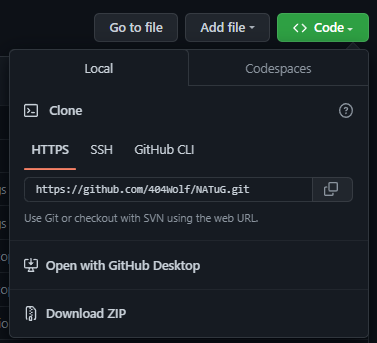
\includegraphics[width=2in]{github-download-menu.png}
		\caption{Github code download menu}
	\end{figure}
	
	\begin{enumerate} \label{sect:getting-natug-running}
		\item Visit \href{Python's download page}{www.python.org/downloads}, and then install the most recent version of Python for your operating system. NATuG has been confirmed to work on versions up to Python 3.11.1
		\item Go to the \href{NATuG’s Github page}{github.com/404Wolf/NATuG}, click the green ``code'' button, and then click ``download ZIP.'' See Figure~\ref{fig:github-download-menu}.
		\item Open your computer's terminal/console/command prompt. Enter the following commands, in the following order. 
		
		\begin{enumerate}
			\item ``\texttt{cd $<$filepath$>$}'' to enter the directory of the project. \label{enum:enter-directory}
			
			\item ``\texttt{python~-m~venv~venv}'' to create a virtual environment for the needed libraries to go into.
			
			\item ``\texttt{venv/Scripts/activate}'' if you are on windows, or ``source~myenv/bin/activate'' if you are on Mac/Linux, to enter into the virtual environment. You will know that you have successfully entered the virtual environment if the current line in terminal begins with ``(venv).'' \label{enum:activate-venv}
			
			\item ``\texttt{python -m pip install -r requirements.txt}'' to automatically install all the needed libraries. They may take a while to download.
			
			\item ``\texttt{python -m launcher}'' to run the program. The first launch may take a bit while the code compiles. \label{enum:run-program}
		\end{enumerate}
	
		\item You should now be in NATuG! When running the program in the future, simply CD into the folder (step~\ref{enum:enter-directory}), enter the virtual environment (step~\ref{enum:activate-venv}), and run the program (step~\ref{enum:run-program}).
	\end{enumerate}

\section{Quickstart}

Constructing a DNA nanotube is a complex, multi-stage process, but NATuG streamlines the steps. Below is a quick list of things to do that should help you gain a basic level familiarity with NATuG.

\textbf{Disclaimer:} The below tasks are by no means comprehensive, and are meant to serve as a simple introduction to the program.

\subsection{Running NATuG}
First, go to Section~\ref{sect:getting-natug-running} and follow the instructions to get NATuG running.

\subsection{Nucleic Acid Selection}

On the right side of the screen, in the config panel, you will find the Nucleic Acid settings tab. This is the area in which settings for the geometry of your DNA. While most of the time you will use NATuG's default profiles for DNA settings (and, most of the time, the MFD B-Type DNA profile), now is a good time to experiment with the different inputs. As you change the different settings, also look at the bottom of the NATuG's window---the Status Bar--when hovering over them. It should display a brief explanation of what the different settings actually are. Observe the Side View Plot and Top View Plot change as the settings update.

\begin{figure}[h] \label{fig:nucleic-acid-tinkering}
	\caption{Experimenting with Nucleic Acid settings}
	\centering
	\begin{subfigure}{.5\textwidth}
		\centering
		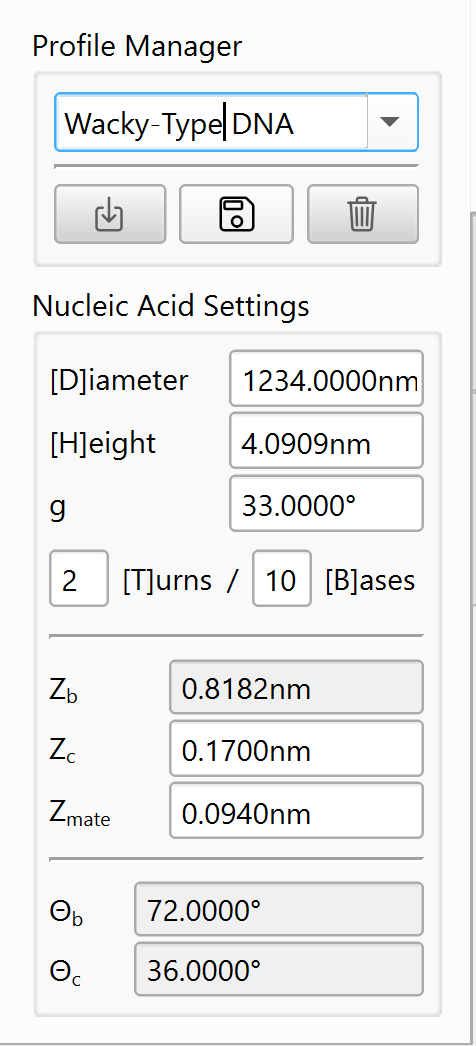
\includegraphics[height=1.7in]{nucleic-acid-tinkering.png}
		\caption{Tinkering With Nucleic Acid Settings}
	\end{subfigure}%
	~
	\begin{subfigure}{.5\textwidth}
		\centering
		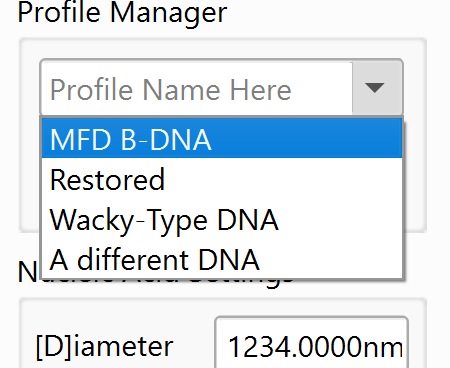
\includegraphics[width=1.7in]{nucleic-acid-tinkering-2.png}
		\caption{Loading different Nucleic Acid profiles}
	\end{subfigure}
\end{figure}
	
\subsection{Domain Adjustment}

In the config panel on the right side of the screen, switch to the Domains tab. The panel will pop out because of the required width of the tab. The panel may appear intimidating at first, but you should start by using the small arrow buttons next to the "m" of each domain. As you do so, watch the Top View Plot update in real time. By increasing/decreasing the "m" values, the interior angles of domains will change, which will in turn change the shape of the tube. You can type numbers directly into the boxes, but without correcting for changes with other domains' angles, the tube will open up. Notice how when the tube is closed the M/R box in the symmetry section of the tab lights up green.

In the settings area above the domains table, click the load button (the button that has an arrow pointing downwards into a box). Choose a different set of domains, for instance, "nested.csv." As you play around with this section of NATuG, you can use the save button to save your own designs/your adjustments to the default designs.
	
\begin{figure}[h] \label{fig:domain-tinkering}
	\caption{Changing up domain settings}
	\centering
	\begin{subfigure}{.5\textwidth}
		\centering
		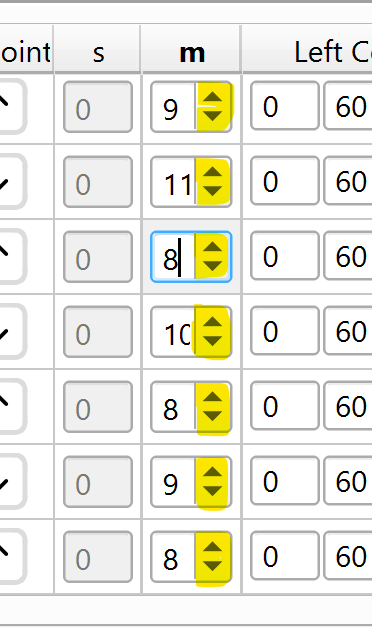
\includegraphics[height=2in]{changing-theta-ms.png}
		\caption{Changing domains' $\theta_{m}$s}
	\end{subfigure}%
	~
	\begin{subfigure}{.5\textwidth}
		\centering
		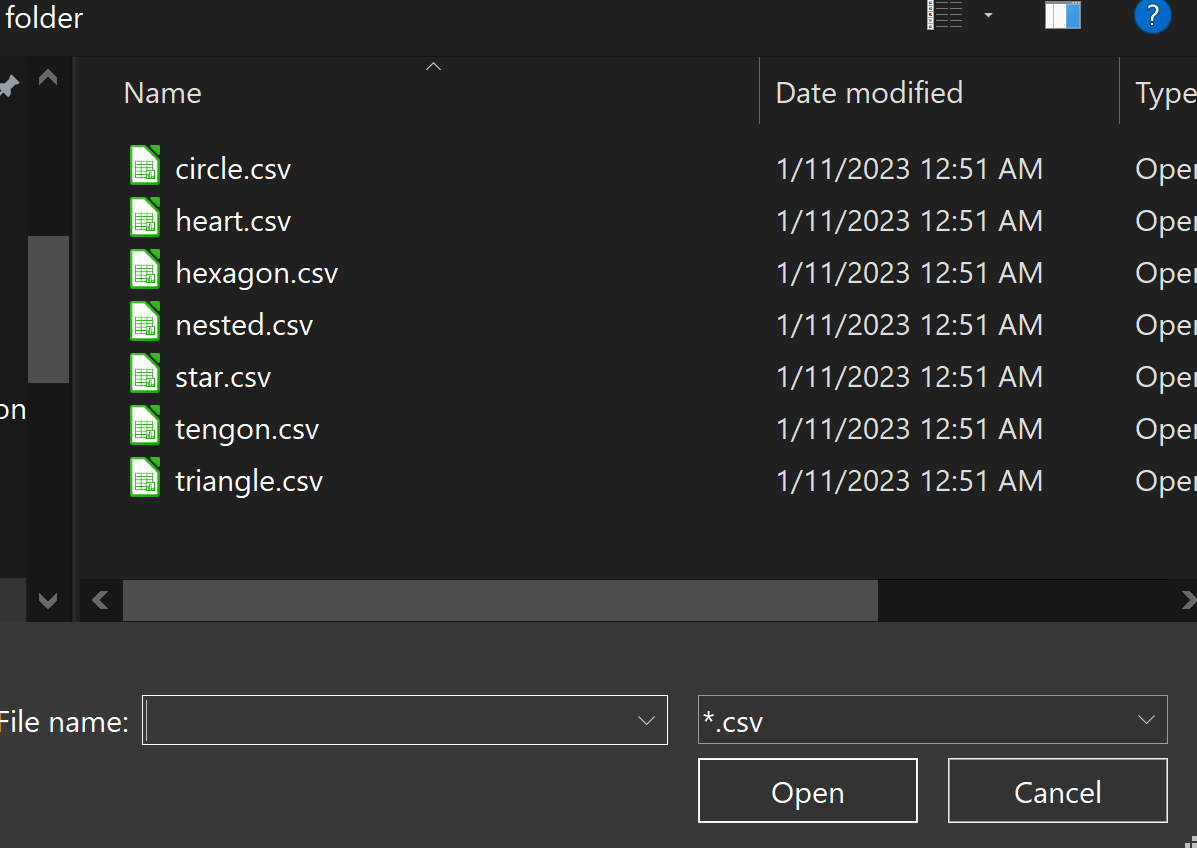
\includegraphics[width=2in]{loading-domains.png}
		\caption{Loading in different domain presets}
	\end{subfigure}
\end{figure}
	
\subsection{Junction Creation} \label{sect:quickstart-junction-creation}
\begin{figure}[h] \label{fig:creating-junctions}
	\centering
	\caption{Creating cross-strand junctions}
	
	\begin{subfigure}{.3\textwidth}
		\centering
		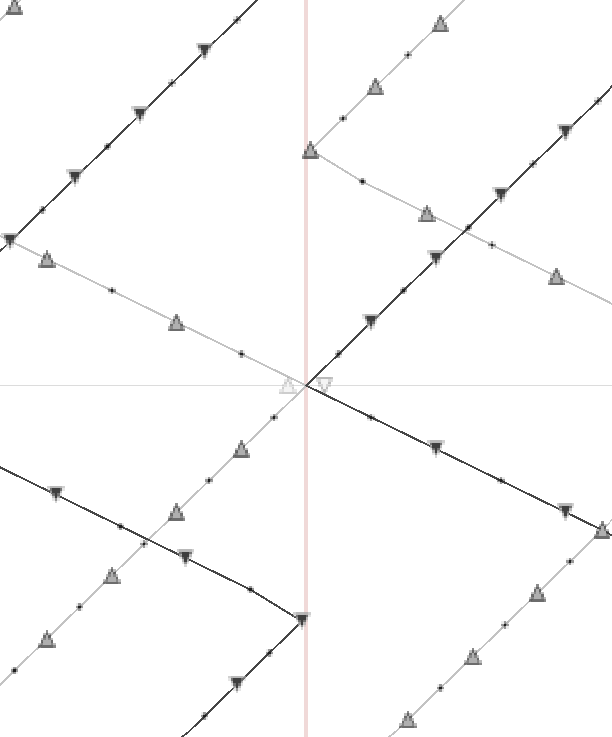
\includegraphics[height=1.7in]{creating-junctions-1.png}
		\caption{Domains with overlapping NEMids}
	\end{subfigure}%
	~
	\begin{subfigure}{.3\textwidth}
		\centering
		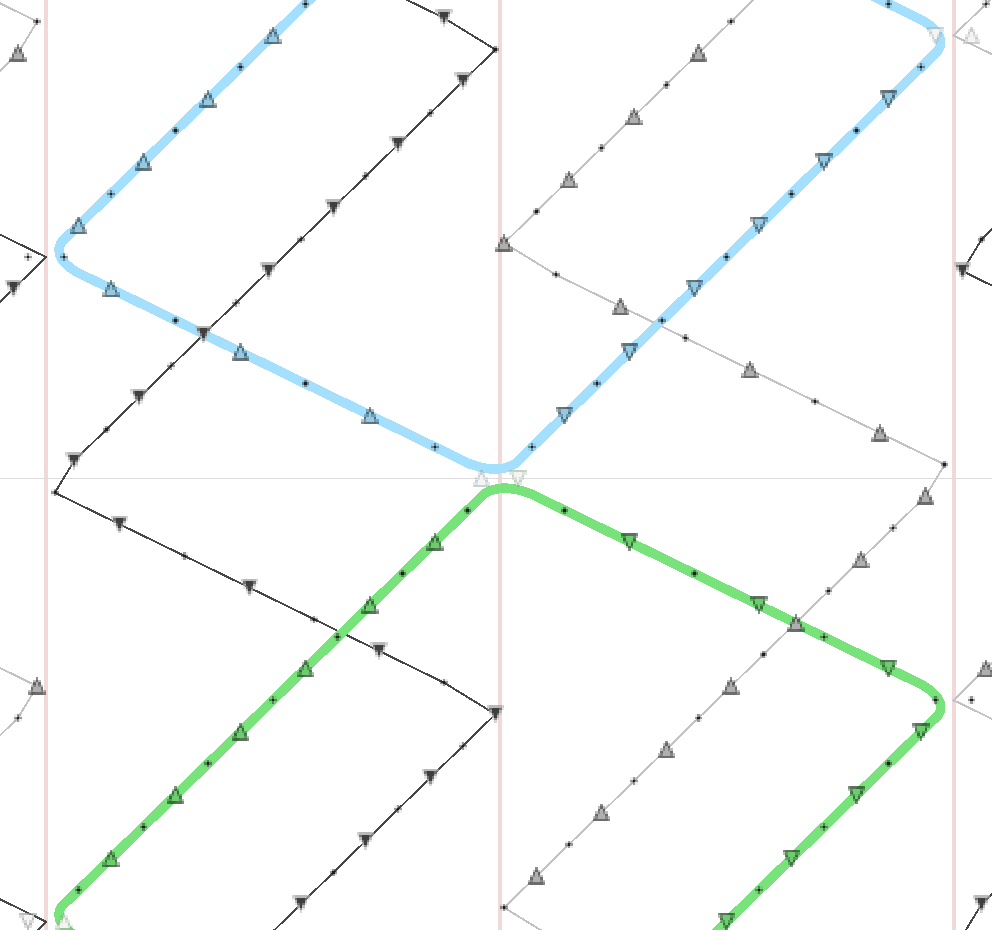
\includegraphics[height=1.7in]{creating-junctions-2.png}
		\caption{Domains with inter-domain strands}
	\end{subfigure}%
	~
	\begin{subfigure}{.3\textwidth}
		\centering
		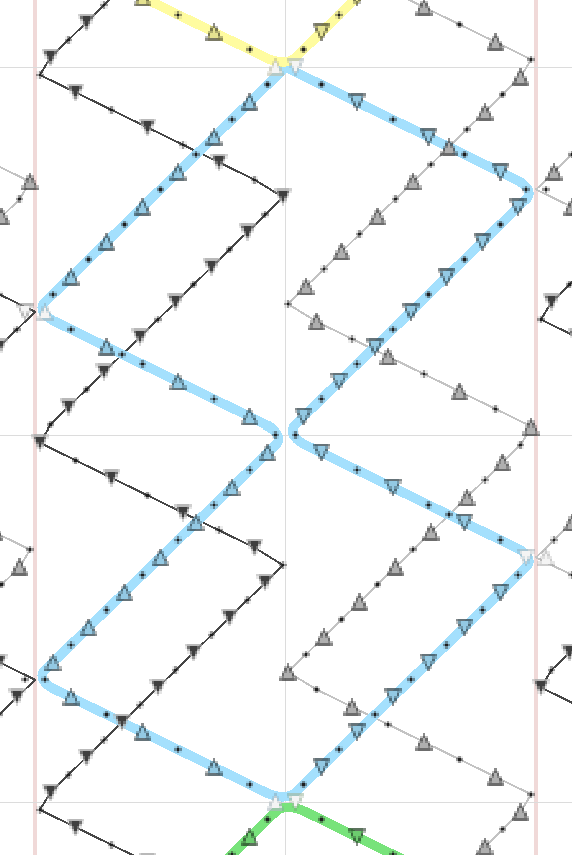
\includegraphics[height=1.7in]{creating-junctions-3.png}
		\caption{Domains with a closed-loop strand and inter-domain strands}
	\end{subfigure}
\end{figure}

In the Side View Plot---the main area of NATuG---locate two white triangles (which represent the middle of two nucleosides, and are called ``NEMids'') that are overlapping, and click on them. This will transform two helices of two different domains into two helices that traverse both of the domains. Continuing clicking on overlapping white triangles to weave together strands. See Figure~\ref{fig:creating-junctions} for a visual example.

\subsection{Nicks, Linkages, and Sequences}
Here, you can begin to experiment with more advanced features of NATuG. You just experimented with creating junctions, but the Side View Plot mode that creates junctions (``juncter'' mode) is only one of many modes (though it's likely the mode you'll be using the most). To try out other modes, go to the top of the window, where you see a list of different buttons (``Informer,'' ``Juncter,'' ``Nicker,'' etc.), and click on different modes. Then left click on points within the main plot. Below is a list of (very) simplified descriptions of the different modes and how to get started using them.

\begin{figure}[h] \label{fig:advanced-NATuG-features}
	\caption{Advanced NATuG features}
	\centering
	\begin{subfigure}{.3\textwidth}
		\centering
		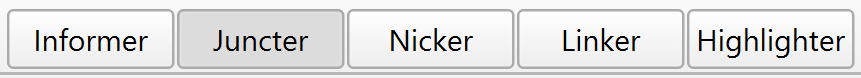
\includegraphics[width=1.4in]{juncter-activated.png}
		\caption{There are other modes!}
	\end{subfigure}%
	~
	\begin{subfigure}{.3\textwidth}
		\centering
		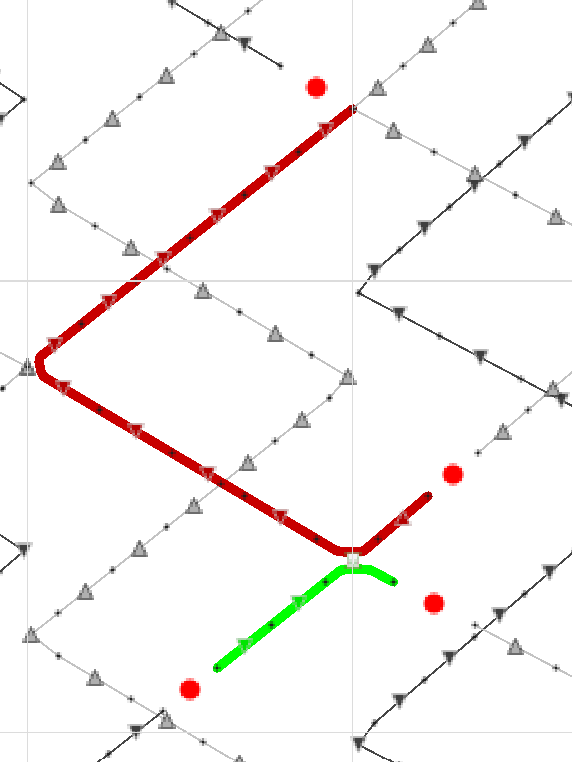
\includegraphics[height=1in]{nick-examples.png}
		\caption{Examples of nicks}
	\end{subfigure}%
	~
	\begin{subfigure}{.3\textwidth}
		\centering
		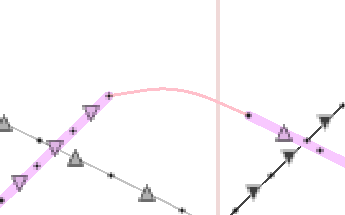
\includegraphics[width=1.5in]{linkage-example.png}
		\caption{Example of linkages}
	\end{subfigure}
\end{figure}

\begin{enumerate}
	\item \textbf{Informer Mode:} Obtain information about points. To use, click on any point.
	\item \textbf{Juncter Mode:} Redirect strands across helical domains. To use, click on any two overlapping white triangles.
	\item \textbf{Nicker Mode:} Split strands in half. To use, click on any point.
	\item \textbf{Linker Mode:} Link the ends of two strands together to make one bigger strand. To use, click on one point that is at the end of a strand, and then another point that is at the end of a strand. Make sure that the arrows do not point towards each other.
	\item \textbf{Highlighter Mode:} Highlight points. To use, click on any point.
\end{enumerate}

\section{Overall Layout}

NATuG’s interface consists of a main hub area, surrounded by two panels. There is a status bar at the bottom of NATuG, which provides helpful descriptions of what various buttons and input boxes do as you hover over them, and a file bar at the top of NATuG, which provides access to various cross-program functions.

 \begin{figure}[h] \label{program-layout}
	\centering
	\caption{The overall layout of NATuG}
	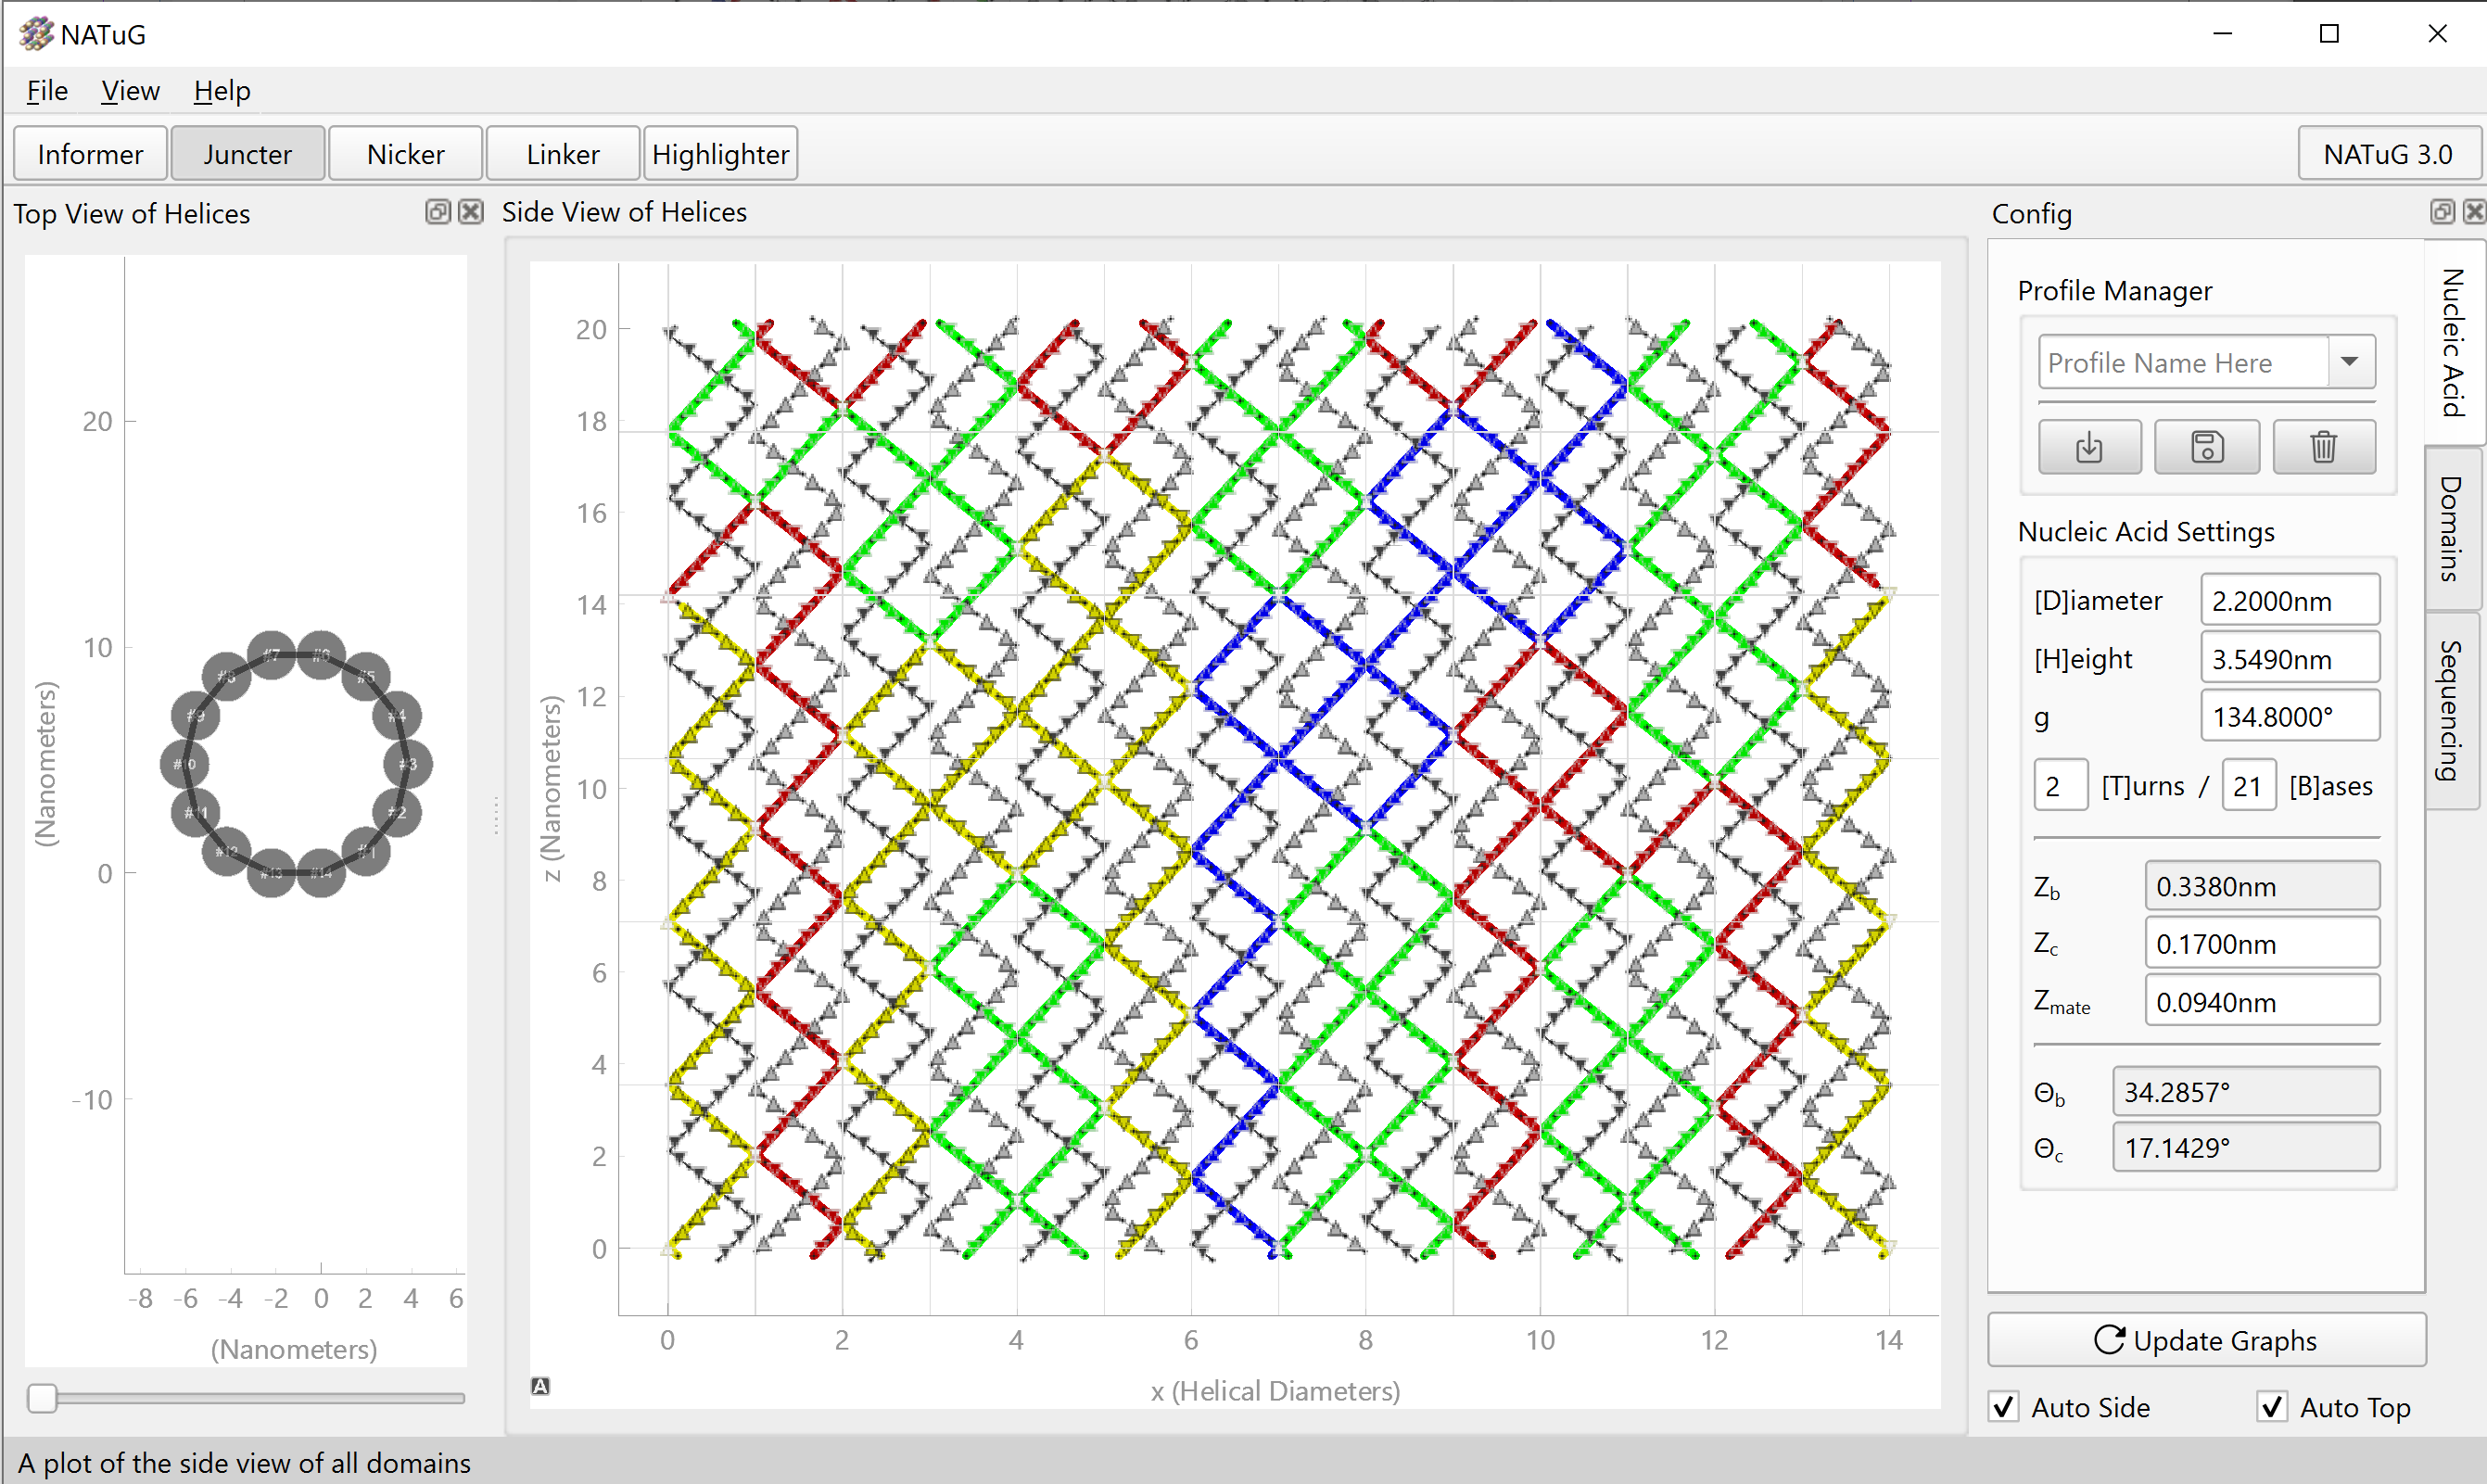
\includegraphics[width=5in]{program-layout.png}
\end{figure}

\subsection{Hub}
NATuG's main area, the “hub,” is another name for the area of the program where the Side View plot is located. Located directly above the Hub is the toolbar, where you can select the current mode of NATuG. Each mode changes what a left click does in the Side View plot.

\subsection{Panels}
NATuG currently has one Panel: the ``config'' panel; however, in the future additional Panels may be added. Some of the important properties of Panel-type widgets are listed below.

\begin{enumerate}
	\item Panels are all undockable. By clicking twice on the top area of a panel, or by dragging the panel away from the main window, or by clicking the  button, one can make a panel become its own window. To redock, click on the top of the panel twice, or drag the panel back into the main window. 
	
	\item Panels are hideable. By clicking the "x" button in the top corner of a panel, or by going to the file menu, "view," and then the name of the panel you are trying to hide, you can hide the panel. To unhide a panel, go to the file menu, "view," and then the name of the panel you are trying to unhide. 
\end{enumerate}

\section{Config Panel} \label{section:config-panel}	
The Config Panel contains most of the user input areas of NATuG. Within the panel are three primary Subpanels: ``\textbf{Nucleic Acid},'' ``\textbf{Domains},'' and ``\textbf{Sequencing},'' and ``\textbf{Snapshots},'' outlined in greater depth on the following pages.

To navigate between Subpanels of the config panel, simply click on one of the tabs on the right. Below are brief descriptions of the various tabs; however, each tab has a dedicated page as well.

\textbf{Warning:} changing settings within the Config Panel will reset all current junctions, nicks, links, and highlights. Attempting to change settings when there exist any junctions, links, or highlights will result in a popup dialog that offers to save the current state of the Side View Plot and then refresh the plot, refresh the plot without saving, or cancel the attempted refresh. Thus, you generally want to configure the geometry of the structure before you interact with the strands.

\begin{figure}[H] \label{fig:nucleic-acid-tab-activated}
	\centering
	\includegraphics[width=3in]{"nucleic-acid-tab-activated.png"}
\end{figure}

The Nucleic Acid Tab is where one can customize the geometrical settings of the nucleic acid that they are creating a nanotube for. They default to settings for a slight variation on B type DNA, and generally does not need to be changed. 

\begin{figure}[H] \label{fig:domains-tab-activated}
	\centering
	\includegraphics[width=3in]{"domains-tab-activated.png"}
\end{figure}

The Domains Tab is where settings for the interior angles, strand switches, and the number of NEMids to generate are inputted. This section allows the user to actually define the shape of the nanotube.

\begin{figure}[H] \label{fig:sequencing-activated}
	\centering
	\includegraphics[width=3in]{"sequencing-tab-activated.png"}
\end{figure}

The Sequencing Tab is where the user can apply bulk sequence actions to all the strands, and export sequences to a spreadsheet for synthesis. This is generally one of the later steps in the nanotube design process.

\begin{figure}[H] \label{fig:snapshots-activated}
	\centering
	\includegraphics[width=3in]{"snapshots-tab-activated.png"}
\end{figure}

The Snapshots Tab is where version history can be found. It lets you rollback to previous program states with ease, and create ``snapshots'' of states at any time.

\subsection{Graph Updating}

By default, as changes are made within the various tabs of the Config Panel the Side View Plot and Top View Plot automatically update. To disable automatic updating for either plot, click either of the ``Auto Side'' or ``Auto Top'' buttons on the bottom of the Config panel. When automatic updating is disabled, the ``Update Graphs'' button must be clicked to refresh the plots. Manual updating can be useful for larger structures that take a long time to load. Note that these automatic update buttons \textbf{only} apply to updates made within the Config Panel, so any changes made via strand interaction (i.e. such as creating junctions or linkages) will cause the plot to refresh to reflect the change made through the interaction, but may not be indicative of the current state of the Config Panel if auto updating is disabled and update plots has not been clicked.

The current tab of the Config Panel determines what is currently plotted in the Side View Plot. When the current tab is either ``Nucleic Acid'' or ``Domains'' NEMids are plotted, and the mode of the Side View Plot is unrestricted. However, when ``Sequencing'' is active, nucleosides are plotted. This difference is easy to notice, since the difference in the plots is that everything is slightly shifted vertically. When nucleosides are currently plotted (and, by extension, the ``Sequencing'' Subpanel is visible), only the ``highlighter'' and ``informer'' modes are enabled within the Side View Plot's toolbar.

\subsection{Nucleic Acid Tab} \label{sect:nucleic-acid-tab}

The Nucleic Acid Tab is the area in which all geometrical settings for the nucleic acid being used can be entered. All of NATuG's computations utilize these constants, so only make changes if you know what you are doing. This tab contains a profile manager for easily loading in sets of settings, and has various fields that warrant extended descriptions. When using NATuG, recall that hovering over fields will show additional information in the Status Bar at the bottom of the window---this feature is particularly useful for the Nucleic Acid Tab because hovering over setting fields shows descriptions in the status bar of what they represent.

\subsubsection{Profile Manager}

The Profile Manager lets you easily save and load various sets of nucleic acid settings. Using NATuG`s profile defaults will ensure that all the settings are correct for the type of DNA you are working with, although you can also create your own profiles for future use.

By default, NATuG includes common profiles, such as one for B type DNA. Profiles are saved internally, and can easily be loaded/retrieved, and .json files containing the profile data can be found within the saves/nucleic\_acid folder. These files are loaded when NATuG is booted, and can be modified directly. Additionally, when NATuG is closed, the last used settings are saved, and are automatically retrieved upon the next launch. The default profiles that ship with NATuG cannot be removed.

The Profile Manager allows you to load profiles, save profiles, and delete profiles. To do so, enter the name of the profile you would like to save/load/delete into the ``Profile Name Here'' box, and click the respective button. Below are extended descriptions of what the three actions do. When a Profile Manager box is disabled/gray, consult the status bar for information as to why (this can happen for various reasons, like trying to delete a default profile). For irreversible actions, such as deleting a profile, warnings will be shown before the action is run that will give you a chance to not do the action. Below are extended descriptions of the various Profile Manager actions.

\begin{figure}
	\caption{Various Profile Actions}
	
	\centering
	\begin{subfigure}{.3\textwidth} \label{fig:load-profile-button}
		\centering
		\caption{The load profile button}
		
\includegraphics[width=1in]{load-profile-button.png}
	\end{subfigure}%
	~
	\begin{subfigure}{.3\textwidth} \label{fig:save-profile-button}
		\centering
		\caption{The save profile button}
		
\includegraphics[width=1in]{save-profile-button.png}
	\end{subfigure}%
	~
	\begin{subfigure}{.3\textwidth} \label{fig:delete-profile-button}
		\centering
		\caption{The delete profile button}
		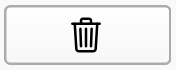
\includegraphics[width=1in]{delete-profile-button.png}
	\end{subfigure}
\end{figure}

\paragraph{Load Profile}
Load the profile with the currently chosen profile name. This requires a profile to already exist with the name chosen, and for the current settings to not be the settings of that profile. (Icon~\ref{fig:load-profile-button})

\paragraph{Save Profile}
Save the profile with the currently chosen profile name, or, if there is already a profile with that name, overwrite the existing profile. The profile will be saved to a \texttt{.json} file within \texttt{saves/nucleic\_acid} after the program is closed. (Icon~\ref{fig:save-profile-button})

\paragraph{Delete Profile}
Delete the profile with the currently chosen profile name. This action is irreversible. Default profiles cannot be deleted. (Icon~\ref{fig:delete-profile-button})

\subsubsection{Setting Descriptions}
Below lies a list of all of the various Nucleic Acid settings that can be adjusted. Certain settings (the ones that are have an "(a)" in the table) are automatically determined based on other settings and cannot be user set. \linebreak

\begin{longtable}{|p{.5in}|p{1in}|p{1in}|p{2.2in}|}
	\caption{\label{tab:setting-descriptions}Nucleic Acid Field Descriptions} \\
	
	Input & Name & Data Type & Description \\
	\hline
	
	$D$ & Diameter & number & The diameter of a given domain in nanometers \\ 
	\hline
	
	$H$ & Height & number & The height of one turn about the helical axes \\ 
	\hline
	
	$g$ & Nucleoside-Mate Angle & number between 0 and 360 & The angle about the helical axis between a nucleoside and its Watson-Crick mate \\ 
	\hline
	
	$T/B$ & Helical Turns per Bases & integers & There are T turns every B bases \\ 
	\hline
	
	$Z_b$ (a) & Base Height & number & The height between two NEMids on a given helix \\ 
	\hline
	
	$Z_c$ & Characteristic Angle & number & The height a helix climbs as it rotates through the characteristic angle \\ 
	\hline
	
	$Z_{mate}$ & Nucleoside-Mate Height & number & Vertical distance between a NEMid and its mate on the other helix. \\ 
	\hline
	
	$\theta_{c}$ (a) & Characteristic Angle & number between 0 and 360 & The smallest angle about the helical axis possible between two NEMids on the same helix. \\ 
	\hline
	
	$\theta_{b}$ (a) & Interbase Angle & number between 0 and 360 & The angle that about the helical axis between two NEMids \\
\end{longtable}

\subsection{Domains Tab}

\begin{figure}[h] \label{fig:domain-config-table-angles}
	\centering
	\caption{Domains Config Table}
	
	\begin{subfigure}{.45\linewidth} \label{fig:domains-config-table-angles-tab}
		\centering
		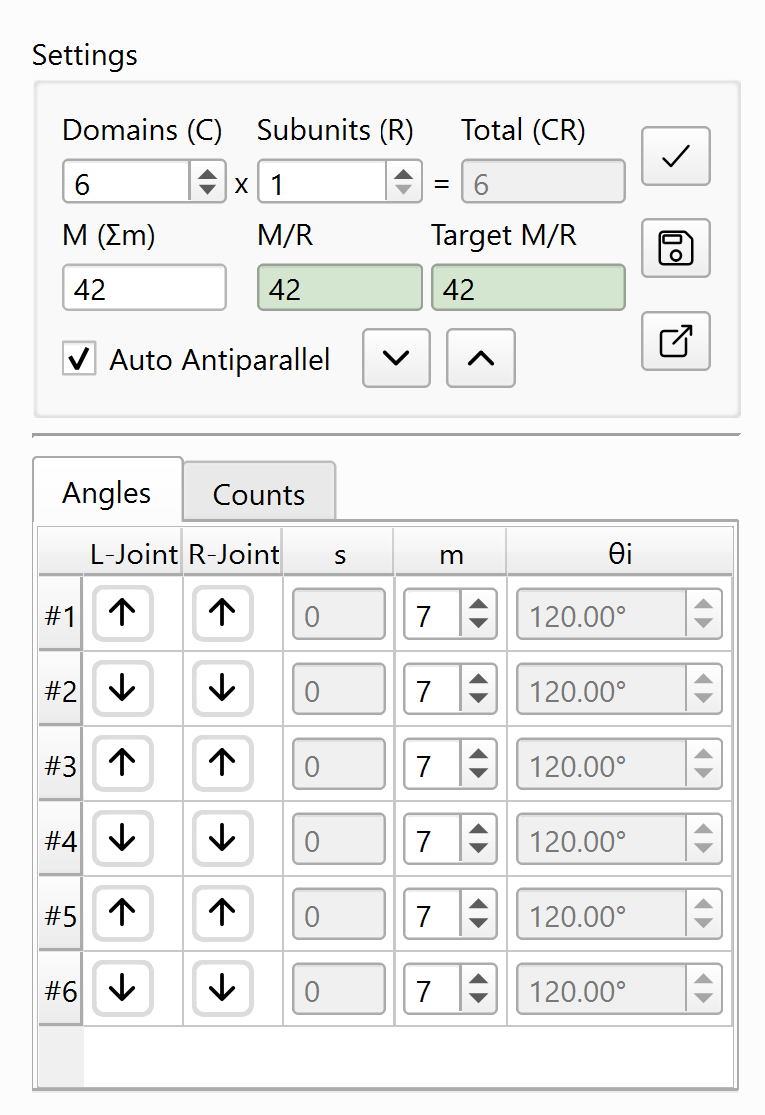
\includegraphics[height=2.5in]{domain-config-table-angles.png}
		\caption{Angles Tab of Domains Config Table}
	\end{subfigure}%
	~
	\begin{subfigure}{.45\linewidth} \label{fig:domains-config-table-counts-tab}
		\centering
		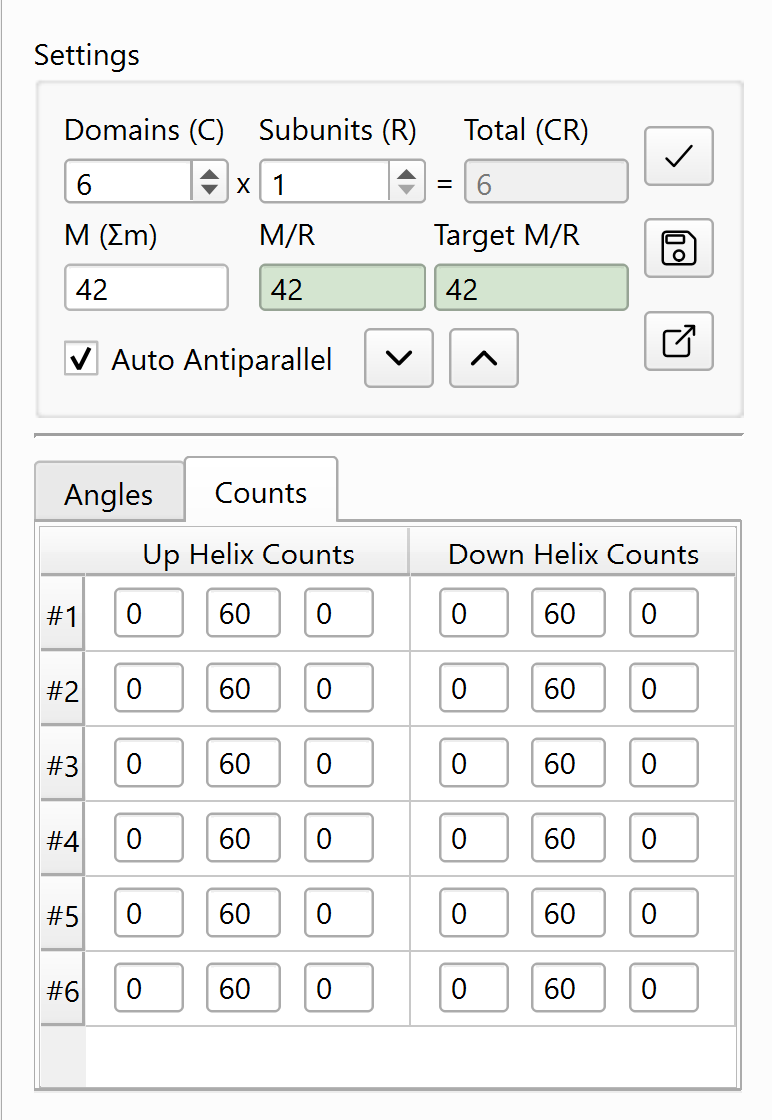
\includegraphics[height=2.5in]{domain-config-table-counts.png}
		\caption{Counts Tab of Domains Config Table}
	\end{subfigure}
\end{figure}

The Domains Tab is the area in which all the settings for each helical domain can be set. The angles between each domain are what determine what the ultimate shape of the nanostructure will be. The ``counts'' are what determine how many nucleosides each strand will be granted. Amongst many other design tools, NATuG allows for designing symmetrical structures, along with the ability to save and load designs. The tab consists of three components: the Settings Area (\ref{fig:domains-tab-settings-area}), Angles Area (\ref{fig:domains-tab-table-angles}), and Counts Area (\ref{fig:domains-tab-table-counts}), all explained in greater detail below.

The Angles Area (\ref{fig:domains-tab-table-angles}) and Counts Area (\ref{fig:domains-tab-table-counts}) are placed within a tabbed area on the bottom part of the Domains Tab, such as not to overwhelm you with too many settings in the same table. Each row corresponds to the same domain, even though columns are bifurcated into two tabs.

\begin{figure} \label{fig:domains-tab-components}
	\caption{Domains Subpanel Components}
	\centering
	\begin{subfigure}{.45\linewidth} \label{fig:domains-tab-settings-area}
		\centering
		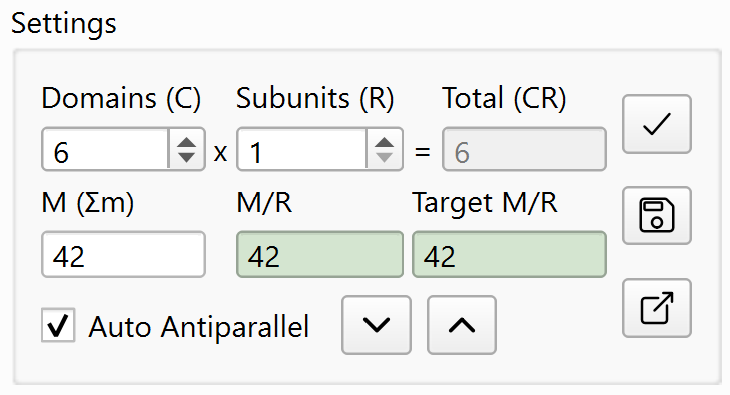
\includegraphics[height=1.5in]{domains-tab-settings-area.png}
		\caption{Settings area}
	\end{subfigure}%
	~
	\begin{subfigure}{.3\linewidth} \label{fig:domains-tab-table-angles}
		\centering
		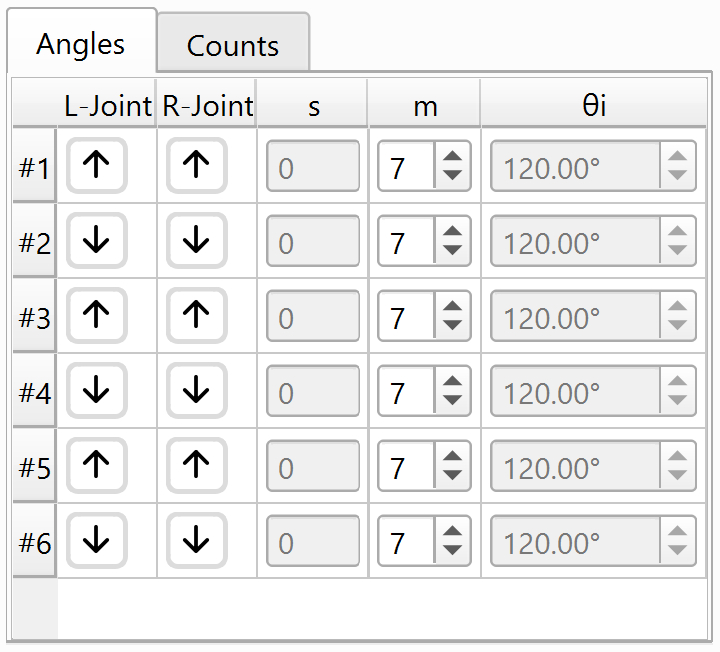
\includegraphics[height=1.5in]{domains-tab-table-angles.png}
		\caption{Angles area}
	\end{subfigure}%
	~
	\begin{subfigure}{.3\linewidth} \label{fig:domains-tab-table-counts}
		\centering
		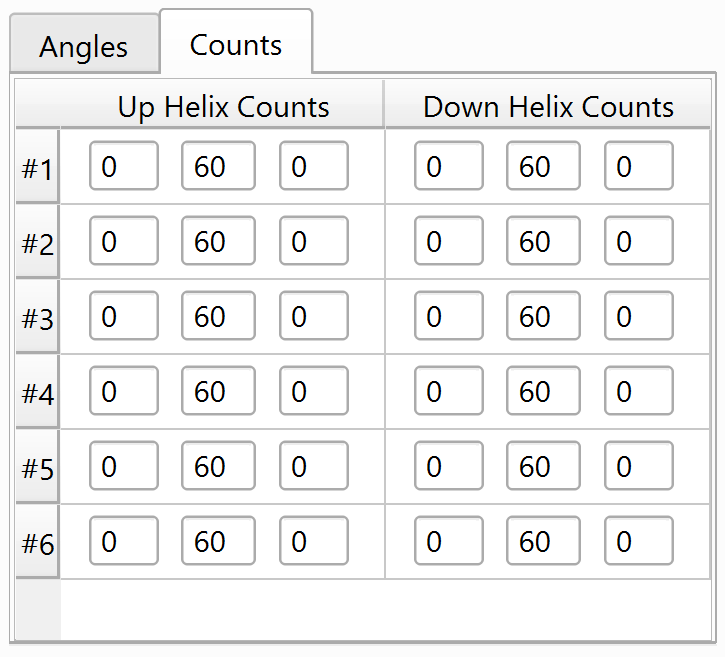
\includegraphics[height=1.5in]{domains-tab-table-counts.png}
		\caption{Counts area}
	\end{subfigure}
\end{figure}

\subsubsection{Settings Area} \label{sect:domains-tab-settings-area}

The settings area's primary purpose is to allow you to set the number of domains for your structure, however it also includes some critical parameters apropos symmetry.

Symmetry is particularly useful for designing closed structures. What it means, simply put, is that the angle and count settings of a cluster, or ``subunit,'' of domains is repeated a certain number of times. Because of this, the Subunit Table (\ref{sect:domains-tab-angles-area} \& \ref{sect:domains-tab-counts-area}) is \textbf{not} a place to enter settings for every single domain, but rather contains the domains of a single subunit; single subunit structures are a special case in which the Subunit Table does showcase the settings of all domains. Within this settings area of the Domains Tab you can change the number of copies of the domains listed in Subunit Table, along with more advanced settings, listed below. 

Once you have made changes within this area, click the check icon, the top button of the group of three buttons on the right, to confirm your choices for the number of domains. If you choose to reduce the number of domains per subunit, a warning will be displayed informing you that the subunit table is to be truncated to allow for the reduction.

\begin{longtable}{|p{.9in}|p{1in}|p{3in}|}
	\caption{Settings Area Fields} \\

	Name & Datatype & Description \\
	\hline
	
	Domains & integer & The number of domains per subunit. This dictates how many domains show up in the Subunit Table. This is also known as the domain count, or $N$ \\
	\hline
	
	Subunits & integer & How many times to copy the current subunit. This is also known as the symmetry factor, or $R$ \\
	\hline
	
	Total & integer & The total number of domains within all subunits. This is equivalent to $R \times C$. \\
	\hline
	
	$M$ & integer & The sum of all the $m$s for all the domains within all the subunits. \\
	\hline
	
	$\frac{M}{R}$ & integer & The sum of all the $m$s for a given subunit. This is equivalent to, as the name implies, $\frac{M}{R}$. \\
	\hline
	
	Target $\frac{M}{R}$ & number & This is equivalent to $B \times \frac{N-2}{2R}$, where B is a parameter of the specific nucleic acid (which can be adjusted within the Nucleic Acid Tab, discussed in more detail in section \ref{sect:nucleic-acid-tab}), $C$ is number of domains, and $R$ is the symmetry factor. If this is not an integer then that means that, by virtue of the chosen $m$s, forming a closed tube is impossible. \\
	\hline
	
	Antiparallel & boolean & Whether the connection between the right joint of the last domain to the left joint of the first domain in the next subunit should be forced to be antiparallel. If this is enabled and this condition is already met, no action is performed. If there is an odd number of subunits it is not possible to alternate parallelity of each subunit and achieve an antiparallel relationship between the right joint of the last domain of each subunit to the next subunit's first domain's left join. If this is the case an error will be raised, and alternation will occur notwithstanding. \\
\end{longtable}

\begin{figure}[h] \label{fig:rotate-domains-arrows}
	\caption{Rotate Domains Buttons}
	\centering
	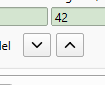
\includegraphics[height=1in]{rotate-domains-arrows.png}
\end{figure}

An additional tool worth noting here is the \textbf{rotate domains buttons}, shown in figure~\ref{fig:rotate-domains-arrows}. These buttons allow you to shift the settings of each domain in the template subunit upwards one, where the first domain's settings take the place of the last domain's settings, or the other way around. These buttons are particularly useful when dealing with non-symmetrical structures.

\subsubsection{Angles Area} \label{sect:domains-tab-angles-area}

The Angles Area of the Domains Subpanel is where you can enter information about the angle of helical domains in relation to other helical domains, along with controlling how the strands align with one another. Each row represents one of the helical domains within the \textbf{first} subunit, and the settings here are copied across all subunits.

\begin{longtable}{|p{.9in}|p{1in}|p{3in}|}
	\caption{Settings Area Fields} \\

	Column & Datatype & Description \\
	\hline
	
	L-Joint & \textit{UP} or \textit{DOWN} & One of the two helices in the double helix is to be lined up to one of the two helices of the previous double helix. This determines whether to align this double helix's up or down helix to the previous domain's double helix. \\
	\hline
	
	R-Joint & \textit{UP} or \textit{DOWN} & Whether to align this double helix's up or down helix to the L-joint helix of the next domain's double helix. \\
	\hline
	
	$s$ & integer & $theta$-switch multiple. This is automatically determined based off of the L-joint and R-joint. $s \in \{-1, 0, 1\}$, and is determined as follows:
	\begin{itemize}
		\item $s=-1$ if the L-joint is \textit{UP} and the R-joint is \textit{DOWN}.
		\item $s=0$ if the L-joint's direction matches that of the R-joint. In this case there is no strand switch.
		\item $s=1$ if the L-joint is \textit{DOWN} and the R-joint is \textit{UP}.
	\end{itemize}
	It's easy to remember because if you're going \textit{UP} to \textit{DOWN} you're doing a negative strand switch, and the same logic applies the other way around.	\\
	\hline
	
	$m$ & integer & The number of characteristic angles between the domain's center and the next domain's center. This is a multiple of $\theta_c$, (which can be set in the Nucleic Acid Tab, discussed in section \ref{sect:nucleic-acid-tab}). While you can manually enter an integer into this box, if you increase the angle of a single domain without compensating elsewhere, the tube will no longer be closed. Clicking the up/down-tick buttons will automatically adjust the interior angle of the surrounding domains, so that this one increases by 2, and the next and previous ones decrease by 1, and vice versa, to maintain the value of $M$. \\
	\hline
	
	$\theta_i$ & number & The actual interior angle between this and the next domain. Equivalent to $\theta_m + \theta_s$, which is also equivalent to $\theta_c*m + \theta_s*s$ \\
\end{longtable}

\subsubsection{Counts Area} \label{sect:domains-tab-counts-area}

The counts area lets you set the number of nucleosides of each strand. All strands are required to begin and end with a nucleoside, with NEMids interspaced between every nucleoside. Because of this, the number of NEMids in each strand is equal to the number of nucleosides in the strand, which can be set in this area of the Domains Tab minus one. 

Like the angles area (\ref{sect:domains-tab-angles-area}), each row represents one of the helical domains within the \textbf{first} subunit, and the settings here are copied across all subunits. The number of nucleosides for the up helix of a given domain in the template subunit can be set by entering values into the respective row of the ``Up Helix Counts'' column. Likewise, you can set the number of nucleosides for the down helix by altering the values of the respective row within the ``Down Helix Counts'' column.

The area wherein you can enter the number of nucleosides you'd like for a given strand takes the form of three integers. They represent the following:

\begin{itemize}
	\item \textbf{Left:} After generating the initial number of nucleosides (set in the middle box), this is how many additional nucleosides to generate and prepend to the bottom of the strand. This can be negative to trim NEMids.
	
	\item \textbf{Middle:} The initial number of nucleosides to generate for the given helix.
	
	\item \textbf{Right:} After generating the initial number of nucleosides (set in the middle box), this is how many additional nucleosides to generate and append to the top of the strand. This can be negative to trim NEMids.
\end{itemize}

Note that adjusting the left and right boxes can be particularly useful for creating sticky ends, since, when the number of additional nucleosides to generate atop a helix does not match that of its complementary helix, there then exist nucleosides that do not have mates (and could theoretically be given bases that correspond with some external viral strand).

\subsection{Sequencing}

\begin{figure}[h] \label{fig:sequencing-tab}
	\centering
	\caption{Sequencing Tab}
	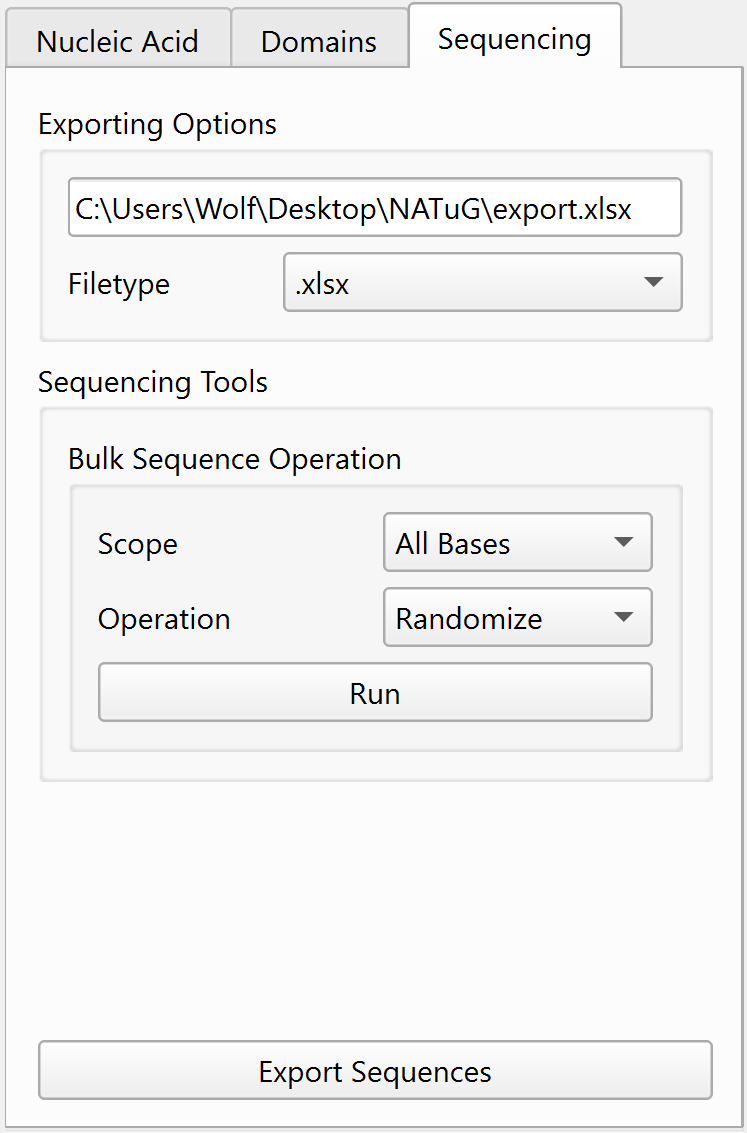
\includegraphics[height=2.4in]{sequencing-tab.png}
\end{figure}

This tab allows for bulk sequence operations, and for exporting sequences to a spreadsheet for synthesis. Because sequencing is such a critical part of NATuG, it has a section that goes into greater depth about how it works. It is also important to note that this is not the only place where sequences can be set. For more information about sequencing, consult section~\ref{sect:sequence-selector}.

\subsubsection{Bulk Sequence Operations}
Bulk sequence operations let you set the sequence of many nucleosides at once. In order to run a bulk sequence operation, select a "Scope," then an "Operation," and then click "Run."

\paragraph{Scopes}
The scope is which nucleosides the operation should run on.

\begin{itemize}
	\item \textbf{All bases:} All the nucleosides of all the strands.
	\item \textbf{Unset bases:} All the nucleosides of all the strands that do not currently have a base set.
\end{itemize}

\paragraph{Operations}
The operation is what to do to the nucleosides within the scope.

\begin{itemize}
	\item \textbf{Randomize:} Select random bases.
	\item \textbf{Clear:} Unset the bases.
\end{itemize}

\section{Side View Plot}
The Side View Plot is the heart of NATuG. It allows you to directly interact with strands that have been created as a result of user inputs set elsewhere. The plot can be broken into a few distinct parts that function together to allow for a high degree of interactivity. 

\begin{figure}[h] \label{fig:short-side-view-overview}
	\centering
	\caption{The Side View Plot \& toolbar}
	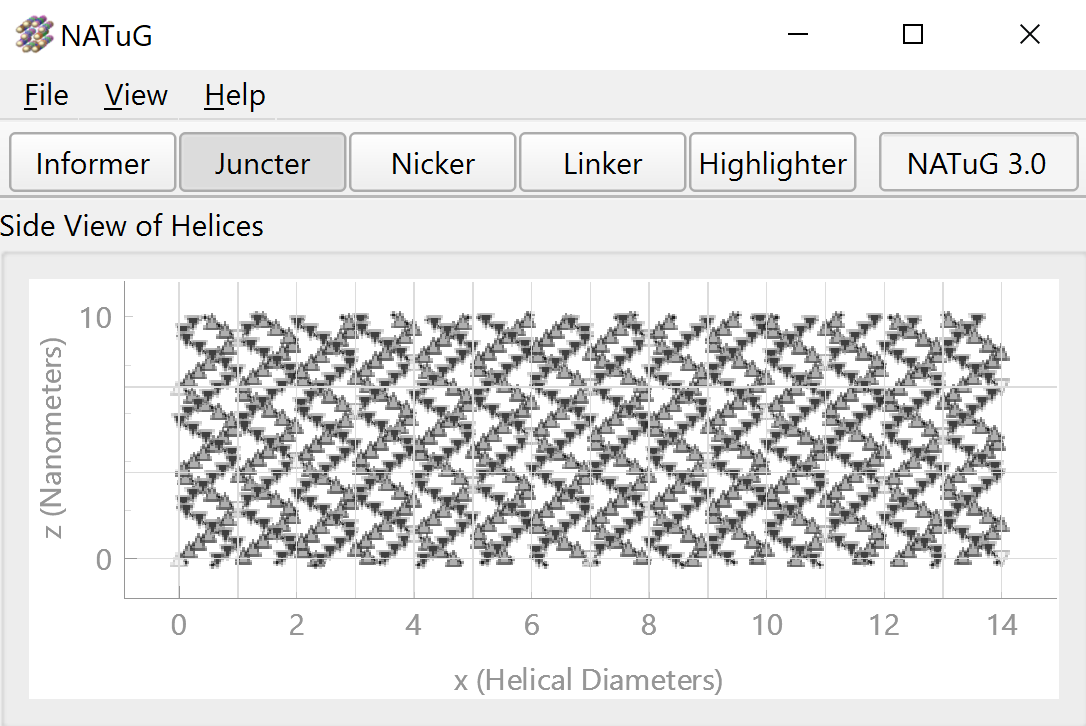
\includegraphics[width=4in]{short-side-view-overview.png}
\end{figure}

\subsection{Graphics}
Before diving into how to actually interact with the Side View Plot, it is important to understand what the contents of the plot actually represent. The Side View Plot is not, as its name suggests, a direct side view of the double helices. Rather, it is more of an ``unrolled'' plot, since it is distorted in such a way as to neatly lay out the double helices next to one another. It is a type of projection.

Importantly, the plot consists of various artifacts, which represent physical nucleosides, or abstract areas between physical nucleosides, NEMids. Below lies further descriptions of what these artifacts appear as.

\subsubsection{Axes}

\paragraph{Axis units}
The $x$ and $y$ axes have labels that indicate their dimension, but the gridlines represent more intuitive concepts.

\begin{itemize}
	\item The x-axis labels represent helical diameters, and thus also define sections between domains. All points between $x=0$ and $x=1$ are in domain\#1, those between $x=1$ and $x=2$ are in domain\#2, and so forth.
	\item The y-axis labels represent the actual vertical height, and the gridlines represent each complete helical twist.
\end{itemize}

\paragraph{Gridlines}

\begin{figure}[H]
	\centering
	\begin{subfigure}{.4\linewidth}
		\centering
		\caption{Unstable join example (0 junctions)}
		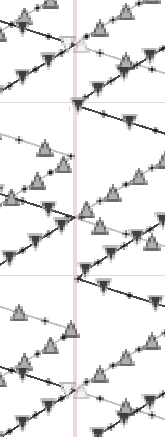
\includegraphics[height=2in]{unstable-joint-example.png}
	\end{subfigure}~
	%
	\begin{subfigure}{.4\linewidth}
		\centering
		\caption{Stable joint example (2 junctions)}
		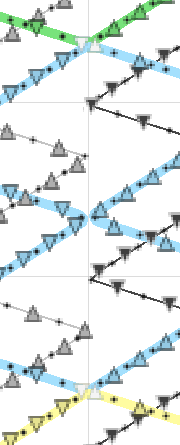
\includegraphics[height=2in]{stable-joint-example.png}
	\end{subfigure}
\end{figure}

The \textbf{horizontal} gridlines lie beginning at $z=0$ and repeat upwards up until the top of the highest point (nucleoside/NEMid). The gridlines themselves are all gray and identical in style.

The \textbf{vertical} gridlines lie beginning at $x=0$ and repeat up until the right of the last helical domain. For each helical joint, including the last one, if there are less than two active junctions the line will appear slightly thicker and red so as to indicate that the joint will be unstable. To make it return to a benign gray, make at least two junctions along the helical joint.

\subsubsection{Points}

\begin{figure}[h] \label{fig:side-view-plot-point-graphics}
	\centering
	\caption{Side View Plot Point Graphics}
	
	\begin{subfigure}{.22\linewidth} \label{fig:up-triangle}
		\centering
		
\includegraphics[width=.3in]{up-triangle.png}
		\caption{Triangle Point}
	\end{subfigure}%
	~
	\begin{subfigure}{.22\linewidth} \label{fig:up-chevron}
		\centering
		
\includegraphics[width=.3in]{up-chevron.png}
		\caption{Chevron Point}
	\end{subfigure}%
	~
	\begin{subfigure}{.22\linewidth} \label{fig:base-symbol}
		\centering
		
\includegraphics[width=.3in]{base-symbol.png}
		\caption{Letter Point}
	\end{subfigure}%
	~
	\begin{subfigure}{.22\linewidth} \label{fig:nondominant-point}
		\centering
		
\includegraphics[width=.3in]{nondominant-point.png}
		\caption{Circle Point}
	\end{subfigure}
\end{figure}

These symbols represent different artifacts, as follows...

\begin{tabular}{|p{2in}|p{4in}|}
	Icon & Artifact \\
	\hline
	
	Triangle & NEMid (the midpoint between two nucleosides) whose direction matches that of the triangle. \\
	\hline
	
	Chevron & Nucleoside with an unset base whose direction matches that of the chevron. \\
	\hline
	
	Letter & Nucleoside with a set base that matches that of the letter, and whose direction is equal to that of the direction that the text reads in. \\
	\hline
	
	Circle & A nucleoside or NEMid that cannot be interacted with. When the Config Panel (\ref{section:config-panel}) is in Sequencing mode only nucleosides can be interacted with, for example, but NEMids are still displayed as small dots. \\
\end{tabular}

\subsubsection{Lines}

\begin{figure}[h] \label{fig:side-view-plot-line-graphics}
	\centering
	\caption{Side View Plot Line Graphics}

	\begin{subfigure}{.4\linewidth} \label{fig:strand-line}
		\centering
		
\includegraphics[width=.3in]{strand-line.png}
		\caption{Default Strand Line}
	\end{subfigure}%
	~
	\begin{subfigure}{.3\linewidth} \label{fig:interdomain-strand-line}
		\centering
		
\includegraphics[width=.3in]{interdomain-strand-line.png}
		\caption{Default Interdomain Strand Line}
	\end{subfigure}
\end{figure}

The lines connecting dots together are not a literal representation of the location of the phosphate backbone of the DNA, but rather serve as a visual aid to see which strands are which. To this end, by default ``interdomain'' strands (strands that traverse multiple domains) are automatically styled to be thicker and more colorful to stand out; however, the styles of lines are completely customizable and need not be this way.

Additionally, for interdomain strands, the lines are curved so that it is clear which strand is which, because with the thicker lines, such as those which interdomain strands posses, strands appear to merge with themselves otherwise. At this time, this setting cannot be disabled.

\subsection{Interaction} \label{sect:plot-interaction}
NATuG utilizes the pyqtgraph framework for its plots. Below lies a general description of the means of interaction for the plot, but, for a more direct and comprehensive breakdown, visit \href{https://pyqtgraph.readthedocs.io/en/latest/user_guide/mouse_interaction.html}{pyqtgraph’s website} (\href{https://pyqtgraph.readthedocs.io/en/latest/user_guide/mouse_interaction.html}{pyqtgraph.readthedocs.io}).

\subsubsection{Panning}
To pan from left to right within the side view plot, left click, and then drag your cursor away from the area that you want to pan to. You can think of this as ``pulling'' the graph towards the cursor. Alternatively, if you have a mouse, you also have the option of clicking the scroll wheel and dragging in the direction that you would like to move the plot in. If you wish to pan horizontally only you can click on the x axis labels and drag left/right, and likewise for vertical panning, but with the z-axis.

\subsubsection{Zooming}

To have the plot automatically zoom in out to showcase all of the items currently plotted, click the small ``A'' symbol in the bottom left of the plot. This is called the ``Auto Range'' button. For zooming in on specific areas of the plot, see below.

\begin{itemize}
	\item If you have a mouse:
		\begin{itemize}
			\item To zoom while maintaining the aspect ratio of the plot, use the scroll wheel.
			\item To zoom without regard for the aspect ratio of the plot, right click, and then drag in the direction that you would like to stretch the plot in. The axes will automatically update.
		\end{itemize}

	\item If you have a trackpad:
		\begin{itemize}
			\item To zoom while maintaining the aspect ratio of the plot, pinch inwards to outwards to zoom in, and outwards to inwards to zoom out.
			\item To zoom without regard for the aspect ratio of the plot, pinch and right click simultaneously. 
		\end{itemize}
\end{itemize}

Also it is worth noting that if you wish to zoom horizontally only you can click on the x axis labels and scroll, and likewise for vertical panning, but with the z-axis.

\subsubsection{Configuration}
For additional options for the plot, right click. Upon right clicking, a small dialog showing additional plot options will show up. This allows for more advanced configuration of how the plot appears.

\subsection{Modes}
The currently chosen mode dictates what left clicks on non-dot points in the Side View Plot does. To change the mode, simply click on the mode that you would like to change to. Only one mode can be chosen at a time, and the currently chosen mode is indicated in a slightly darker gray than the others.

\subsubsection{Informer Mode}

\begin{figure}[h]
	\caption{Informer Dialogs}
	\centering
	\begin{subfigure}{.3\textheight} \label{fig:NEMid-informer}
		\centering
		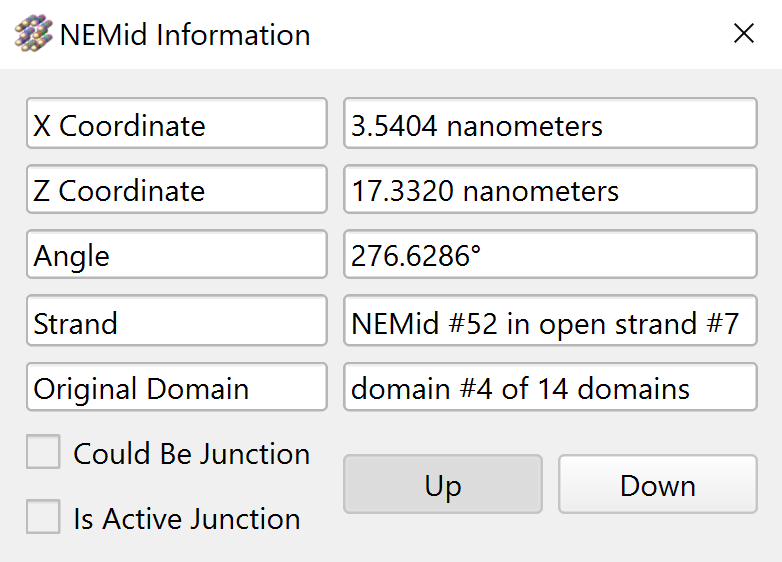
\includegraphics[height=1.3in]{NEMid-informer.png}
		\caption{NEMid Informer Dialog}
	\end{subfigure}%
	~
	\begin{subfigure}{.3\textheight} \label{fig:nucleoside-informer}
		\centering
		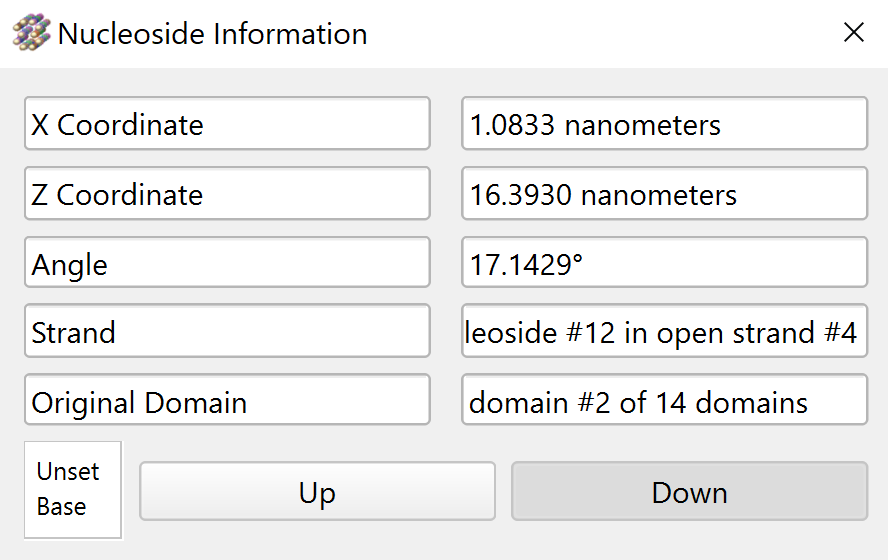
\includegraphics[height=1.3in]{nucleoside-informer.png}
		\caption{Nucleoside Informer Dialog}
	\end{subfigure}
\end{figure}

The "Informer" mode is for obtaining additional information about given points. It provides a dialog that shows various attributes of the point(s) that were clicked on.

The informer mode is for obtaining additional information about given points. When the informer mode is active, clicking on any point within the main plot will create a dialog that provides additional information about the point. If you click on a NEMid that could be made into a junction, two informers will appear---one for the NEMid that was clicked, and one for the NEMid that that NEMid could potentially be made into a junction with. There are two different types of dialogs: the NEMid Dialog~\ref{fig:NEMid-informer} and the Nucleoside Dialog~\ref{fig:nucleoside-informer}.

\paragraph{Nucleoside Informer} \label{paragraph:nucleoside-informer}
Descriptions of the various properties that the Nucleoside Informer displays:
\begin{enumerate}
	\item \textbf{X Coordinate:} The x coordinate of the nucleoside. \label{item:nucleoside-informer-x-coord}
	
	\item \textbf{Z Coordinate:} The z coordinate of the nucleoside. \label{item:nucleoside-informer-z-coord}
	
	\item \textbf{Angle:} The angle of the nucleoside. The line of tangency between the previous domain and this domain marks the zero degree mark. This is automatically moduloed by 360. \label{item:nucleoside-informer-angle}
	
	\item \textbf{Strand:} The index of the nucleoside within its parent strand, and the index of the parent strand within the list of all strands. Indexes begin at \#1. This is the nucleoside index, not the item index, so even though it is true that strands progress nucleoside, NEMid, nucleoside, etc., this index only takes into account nucleosides. \label{item:nucleoside-informer-strand}
	
	\item \textbf{Original Domain:} The domain that this nucleoside belongs to. \label{item:nucleoside-informer-domain}
	
	\item \textbf{Base:} The base that this nucleoside is currently set to. If the nucleoside does not have a base set, this box will read "Unset Base."
	
	\item \textbf{Direction:} The direction of the strand. The darker box is the direction that the strand is going in.  \label{item:nucleoside-informer-direction}
\end{enumerate}

\paragraph{NEMid Informer}
Descriptions of the various properties that the NEMid Informer displays:
\begin{enumerate}
	\item \textbf{X Coordinate:} Same as Nucleoside Informer \#\ref{item:nucleoside-informer-x-coord}
	
	\item \textbf{Z Coordinate:} Same as Nucleoside Informer \#\ref{item:nucleoside-informer-z-coord}
	
	\item \textbf{Angle:} Same as Nucleoside Informer \#\ref{item:nucleoside-informer-angle}
	
	\item \textbf{Strand:} Same as Nucleoside Informer \#\ref{item:nucleoside-informer-strand}
	
	\item \textbf{Original Domain:} Same as Nucleoside Informer \#\ref{item:nucleoside-informer-domain}
	
	\item \textbf{Could Be Junction:} Whether this NEMid could be conjuncted with another NEMid. If this is set to true then clicking on this NEMid in Juncter Mode (\ref{sect:juncter}) will be allowed, otherwise an error will be displayed
	
	\item \textbf{Is Active Junction:} Whether this NEMid is currently conjuncted with another NEMid. 
	
	\item \textbf{Direction:} Same as Nucleoside Informer \#\ref{item:nucleoside-informer-direction}
\end{enumerate}

\subsubsection{Juncter Mode} \label{sect:juncter}

\begin{figure}[h] \label{fig:junction-sites}
	\caption{Junction Sites and Junctable Regions}
	
	\begin{subfigure}{.23\linewidth} \label{fig:junctable-region}
		\centering
		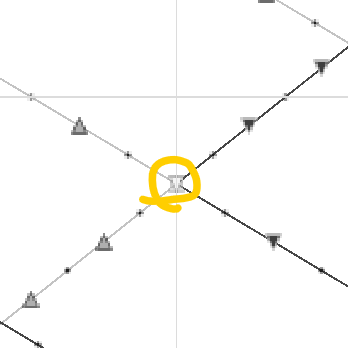
\includegraphics[height=.6in]{junctable-region.png}
		\caption{Two overlaping NEMids}
	\end{subfigure}%
	~
	\begin{subfigure}{.234\linewidth} \label{fig:cross-screen-junctable}
		\centering
		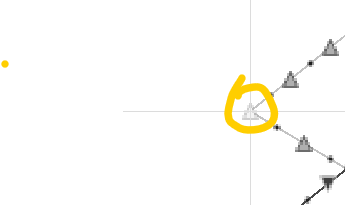
\includegraphics[height=.6in]{cross-screen-junctable.png}
		\caption{Two overlapping cross-screen NEMids}
	\end{subfigure}%
	~
	\begin{subfigure}{.23\linewidth} \label{fig:active-junction-site}
		\centering
		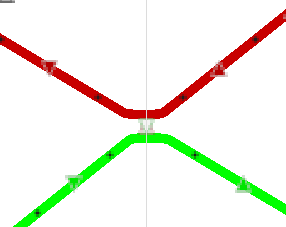
\includegraphics[height=.6in]{active-junction.png}
		\caption{An active junction site}
	\end{subfigure}%
	~
	\begin{subfigure}{.23\linewidth} \label{fig:active-cross-screen-junction}
		\centering
		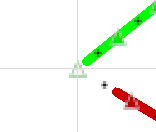
\includegraphics[height=.6in]{cross-screen-junction-site.png}
		\caption{An active cross-screen junction site}
	\end{subfigure}

\end{figure}

The "Juncter" mode allows for the creation of cross-strand exchanges. It lets you left click on overlapping NEMids to create junctions. 

There are two ways to create a junction:
\begin{itemize}
	\item Clicking on two overlapping NEMids (indicated by white triangles that are on top of each other as shown in figure~\ref{fig:junctable-region}). This is the typical type of junction, and is highly versatile---it can split closed loops, form closed loops, allow a strand to go across many domains, and more. See figure~\ref{fig:active-junction-site} for an example of what a junction will look like after a left click.
	\item Clicking on a single NEMid that overlaps a NEMid on the other side of the screen (see figure~\ref{fig:cross-screen-junctable}). This type of junction is called a "cross-screen" junction, and can be seen in figure~\ref{fig:active-cross-screen-junction}. Since the Side View Plot is really an unrolled view of all of the helical domains, the very left for closed structures will sometimes have NEMid overlaps with the very right. 
\end{itemize}

\subsubsection{Nicker Mode}

\begin{figure}[h] \label{fig:nick-examples}
	\centering
	\caption{Nick examples}
	
	\begin{subfigure}{.4\linewidth}
		\centering
		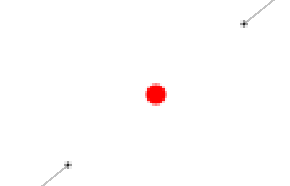
\includegraphics[height=.6in]{nick.png}
		\caption{A nick}
	\end{subfigure}%
	~
	\begin{subfigure}{.4\linewidth}
		\centering
		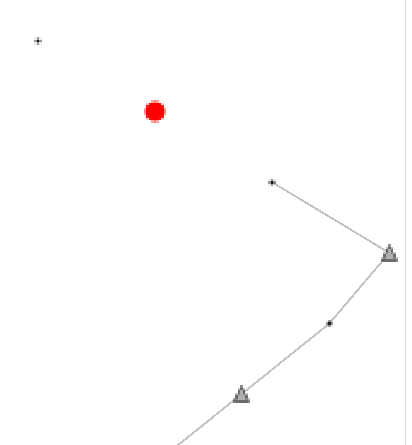
\includegraphics[height=.6in]{end-of-strand-nick.png}
		\caption{A nick at the end of a strand.}
	\end{subfigure}
\end{figure}

The "Nicker" mode is how you can create nicks within the strand. Nicks are essentially gaps that split a strand into two different strands.

To create a nick, click on any NEMid, and the NEMid will convert into a red circle. There will then be two strands: one consisting of all of the NEMids and nucleosides that were above the NEMid, and one consisting of all the NEMids and nucleosides below the NEMid. The NEMid itself will be removed.

Notes about nicking:
\begin{itemize}
	\item When you create a nick the data of the original strand is saved, so, to remove a nick, click on the nick a second time and the original strand will return.
	\item Creating a nick at the end of a strand is unadvised because, as can be seen in figure~\ref{fig:end-of-strand-nick}, you will likely inadvertently create a strand that consists of a single nucleoside.
	\item The nitrogenous bases of all the nucleosides in the two new strands will be preserved.
\end{itemize}

\subsubsection{Linker Mode}

\begin{figure}[h] \label{fig:linkage-editor}
	\centering
	\caption{The linkage editor}
	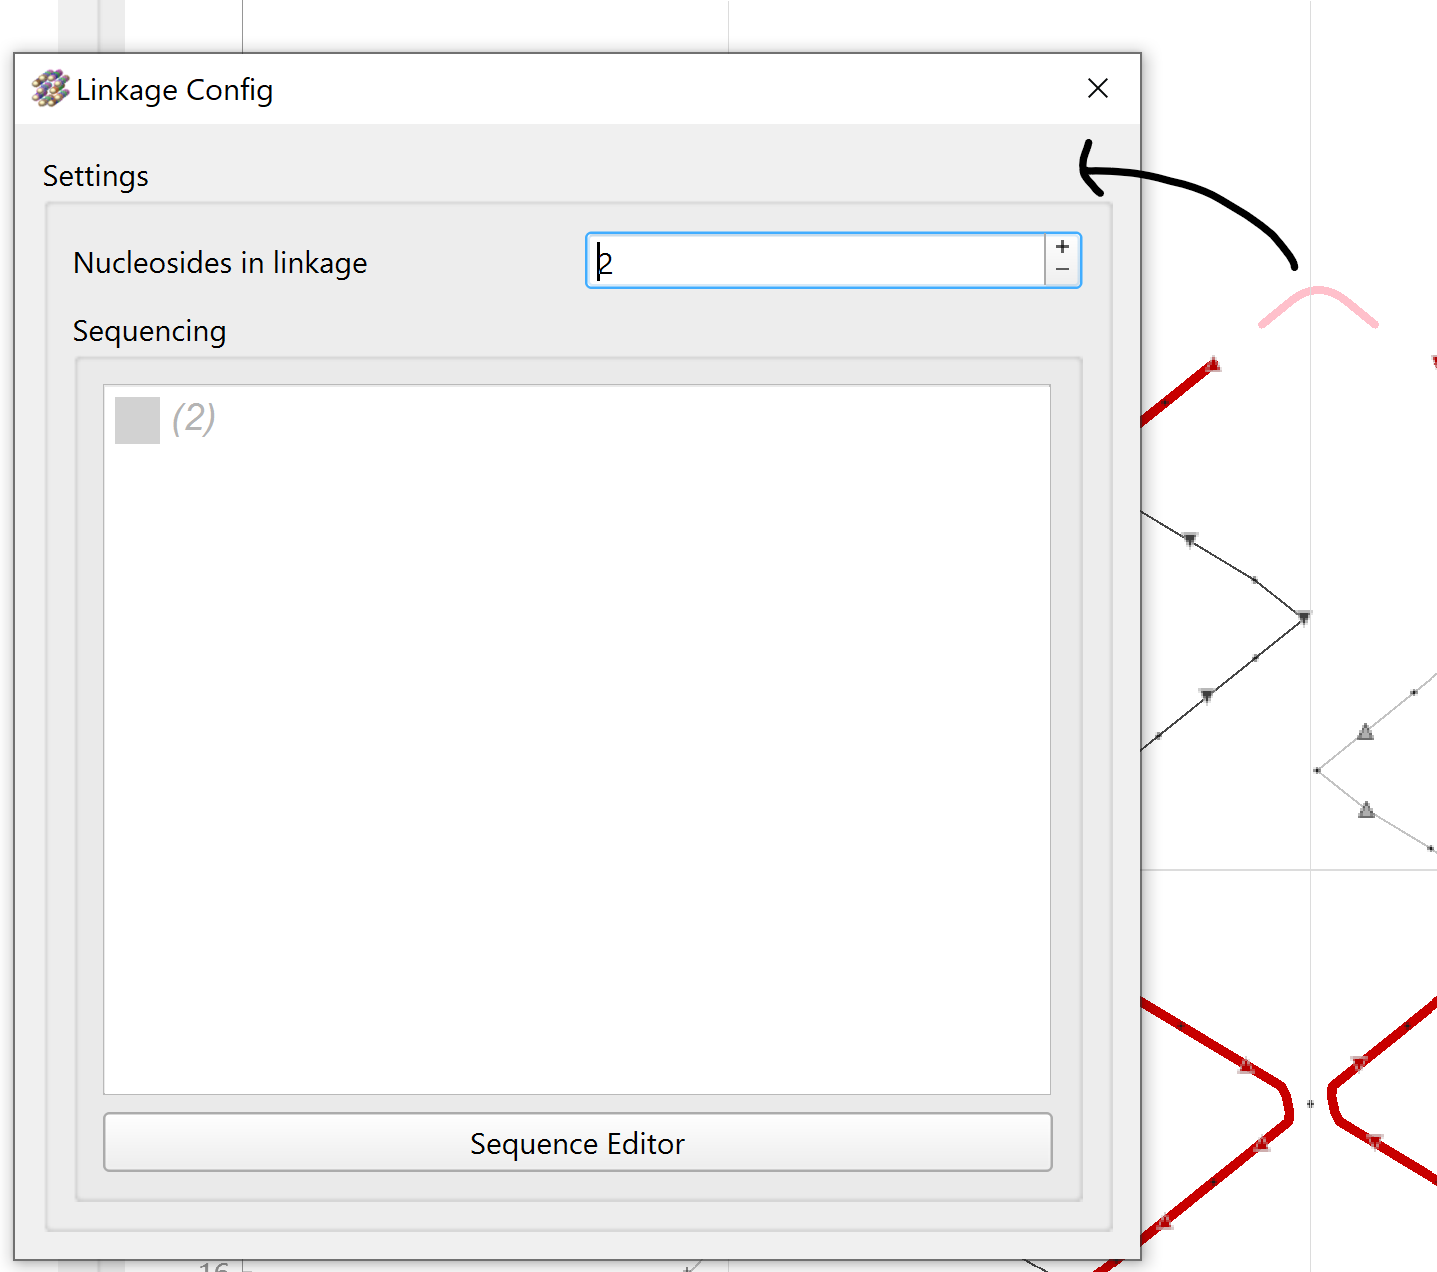
\includegraphics[width=2.3in]{linkage-editor.png}
\end{figure}

The "Linker" mode allows you to connect the end of one strand to the beginning of another strand, and vice versa. 

\paragraph{Linkages}
A linkage is a single-stranded region that connects two formerly distinct strands. In this single-stranded region nucleosides can be added, and bases for those nucleosides can be set. To customize a linkage click on the linkage, and the linkage editor should pop up. The Linkage Editor (see figure~\ref{fig:linkage-editor}) is a dialog that allows you to add nucleosides to the linkage, and to set the sequence of the items in the linkage. To increase or decrease the number of items within the linkage, simply increase the "Nucleosides in Linkage" spinbox, and click tab or enter. Note that the nucleosides in the linkage will show up in the regular strand config sequence editor, but this window only shows the sequence of the items within the linkage.

\begin{figure}[h] \label{fig:linkage-creation-process}
	\centering
	\caption{Linkage creation process}
	
	\begin{subfigure}{.3\linewidth} \label{fig:nick}
		\centering
		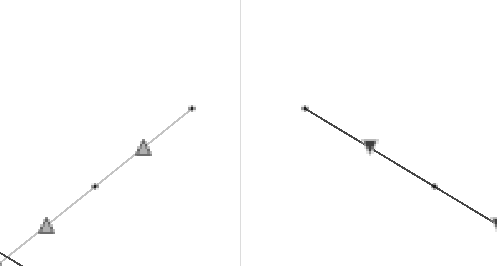
\includegraphics[height=.6in]{pre-linkage.png}
		\caption{Two NEMids that can be linked together}
	\end{subfigure}%
	~
	\begin{subfigure}{.3\linewidth} \label{fig:nick}
		\centering
		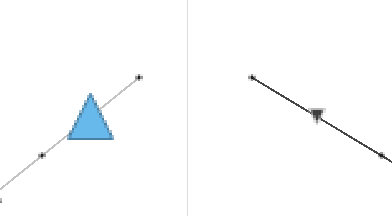
\includegraphics[height=.6in]{pre-linkage-1.png}
		\caption{A selected NEMid that can be linked to another NEMid}
	\end{subfigure}%
	~
	\begin{subfigure}{.3\linewidth} \label{fig:end-of-strand-nick}
		\centering
		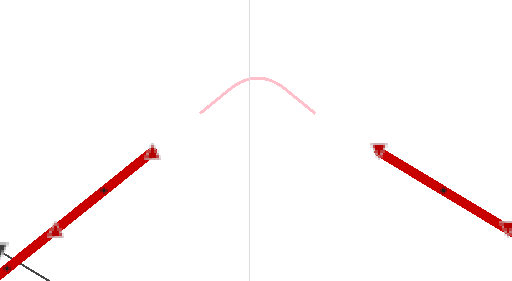
\includegraphics[height=.6in]{linked.png}
		\caption{A completed linkage. This is now one strand.}
	\end{subfigure}
\end{figure}

To create a linkage:
\begin{enumerate}
	\item Locate two NEMids that can be made into a linkage. Consult the following list of prerequisites for determining if two NEMids can be linked together---if the following conditions are not met a warning will be displayed.
	\begin{enumerate}
		\item Both NEMids must be endpoints of their respective strands. This means the second to last or second item in their strands (with the nucleoside that follows them being the very last or very first item).
		\item One NEMid is at the 5' end of its strand and the other NEMid is at the 3' end of its strand.
		\item Both strands consist of $>$1 NEMids.
	\end{enumerate}

	\item Left click on one of the NEMids that you would like to link with the other NEMid. The order in which you click the NEMids does not matter. After clicking on a NEMid in linker mode, the NEMid should turn blue and grow larger. This indicates that it is selected.
	
	\item Left click on the other NEMid that you would like to link it to. A linkage should be created upon releasing left click.
\end{enumerate}

\begin{wrapfigure}{r}{.3\linewidth} \label{fig:highlighted-NEMid}
	\centering
	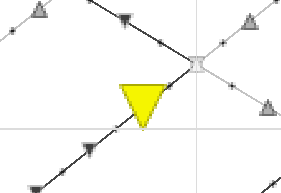
\includegraphics[width=1in]{highlighted-nemid.png}
	\caption{"A highlighted NEMid}
\end{wrapfigure}

\subsubsection{Highlighter Mode}

The "Highlighter" mode lets you highlight points. It makes them larger and yellow, which can be useful for presentations (see figure~\ref{fig:highlighted-NEMid}). 
To highlight a NEMid or nucleoside, simply click on it. To unhiglight a NEMid or nucleoside, click on the highlighted NEMid or nucleoside a second time.

Notes about highlighting:
\begin{itemize}
	\item Items will stay highlighted even when you leave highlighter mode. This means that there are actually multiple ways to unhighlight items, including, but not limited to the following.
	\begin{itemize}
		\item Click the highlighted point while in highlighter mode
		\item Create a nick to split the strand in two, or create junction
		\item Click the "Update Graphs" button to refresh the plots
	\end{itemize}

	\item At this time NATuG's highlighting is uncustomizable, so all higlighted items will be large and yellow versions of their past selves.
\end{itemize}

\subsection{Repetition}

\begin{figure}
	\centering
	\caption{Enabling the Action Repeater}
	\begin{subfigure}{.3\linewidth}
		\centering
		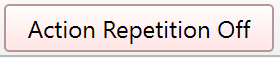
\includegraphics[width=1.9in]{action-repeater-disabled.png}
		\caption{Action repeater disabled}
	\end{subfigure}%
	~
	\begin{subfigure}{.4\linewidth}
		\centering
		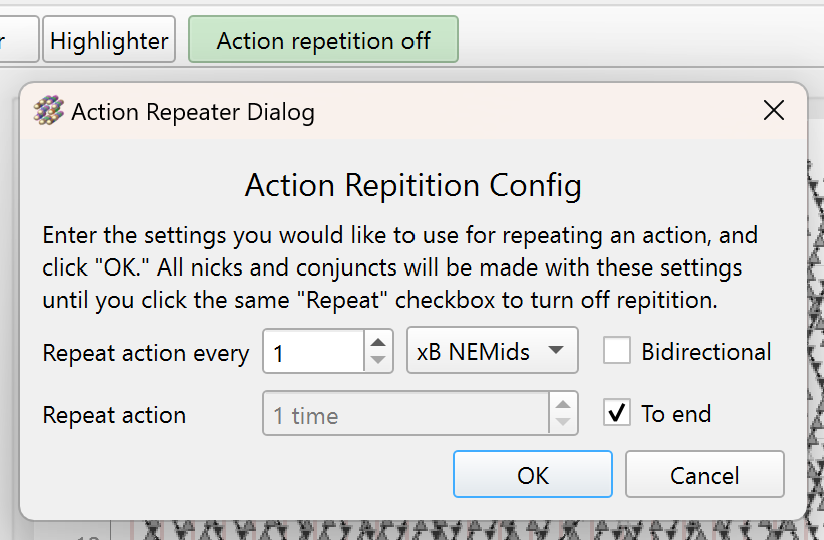
\includegraphics[width=2.5in]{action-repeater-enablement.png}
		\caption{Action Repeater Dialog}
	\end{subfigure}%
	~
	\begin{subfigure}{.3\linewidth}
		\centering
		\includegraphics[width=1.9in]{action-repeater-enabled.png}
		\caption{Action repeater enabled}
	\end{subfigure}
\end{figure}

Often for larger structures, especially ones where helices contain many bases, you will find yourself tediously making junctions all the way up the helices every where and there. Thankfully, NATuG has a tool to streamline the process. With the Action Repeater, you can automatically repeat an action, such as creating junctions, along a \textbf{helix}, with the frequency of your choice. It is important to realize that the action repeater does not repeat actions across strands, but rather traverses up/down \textbf{helices}.

To enable the Action Repeater, click on the large, red button that says ``Action Repetition Off,'' at the top of the screen. Clicking on it should spawn an Action Repetition Dialog, allowing you to configure and then enable the tool. The Action Repeater works for any mode, such as Nicking and Juncting, but if it fails to perform an action at any given point along the helix it is repeating over, it will suppress the error. Within the Action Repeater Dialog there are various settings you can configure, which should be mostly intuitive. You can choose to repeat the action every certain amount of NEMids, or every certain multiple of $B$ (a configurable setting in the Nucleic Acid Profile) NEMids. You can also specify how far up the helix to go in those intervals, or can choose to continue to the end of the strand. Choosing the bidirectional checkbox will make it so that the action repeats up and down the strand (whereas normally it only repeats in the direction of the point you click, up until the end of the strand).

After enabling the Action Repeater, the large red button will turn green and display the current repetition settings. To disable the Action Repeater, simply click the large green button displaying the settings.

\section{Top View Plot}

The Top View Plot presents an overhead view of the nanostructure that is currently being created. It allows you to visualize the actual tube shape, and see the interior angles of all the domains. The Top View Plot is a panel, which means that it can be undocked, among other things. For information on panels, see~\ref{sect:panels}.

\begin{figure}[h] \label{fig:top-view-plot-panel}
	\centering
	\caption{Top View Plot Panel}
	\begin{subfigure}{.45\linewidth} \label{fig:top-view-plot-panel-1}
		\centering
		\includegraphics[width=1.8in]{top-view-plot.png}
		\caption{Top View Plot Example 1}
	\end{subfigure}%
	~
	\begin{subfigure}{.45\linewidth} \label{fig:top-view-plot-panel-2}
		\centering
		\includegraphics[width=1.8in]{top-view-plot-2.png}
		\caption{Top View Plot Example 2}
	\end{subfigure}
\end{figure}

\subsection{Graphics}
In the Top View Plot, each circle represents a helical domain, which is the region in which the double helices exist. The circles are numbered, and the numbers represent the domains' respective indexes. The units of the axes are in nanometers, and depend on the diameter of domains, which can be set in the Nucleic Acid Tab (\ref{sect:nucleic-acid-tab}). An imaginary $0^{th}$ domain is drawn as well to show the last domain's interior angle, but this domain does not actually exist. Additionally, to make it easier to see the interior angles of the domains, a thin line is drawn atop all of the domains' circles.

\subsection{Interaction}
For the most part, interacting with the Top View Plot is the same as interacting with the Side View Plot (documentation for interaction with the side view plot can be found at~\ref{sect:plot-interaction}). However, there are a few important differences:
\begin{itemize}
	\item The aspect ratio of the Top View Plot is locked at 1:1. This means that you cannot stretch the plot.
	\item The Top View Plot is rotatable. To rotate the top view plot, drag the handlebar beneath the plot to the right. The left edge of the bar represents a $0^{\circ}$ rotation, and the right edge of the bar represents a $360^{\circ}$ rotation. The plot is rotated after coordinates for all of the domains are computed, and the pivot point of rotation is the middle point of all the domains.
	\item Clicking on a number (not a circle, but rather on a number) will navigate the Side View Plot to the specific domain that was clicked on. Clicking on the same number a second time will restore the full view of the plot.
\end{itemize}

\section{Saving}

A vital feature of NATuG is the ability to save and load the current program state at any time. NATuG makes this extremely simple: either use \texttt{Control+S}, or go to file, save. Your save will take the form of a \texttt{.natug} file, which contains the entire program state, with the exception of current snapshots, which are their own save files and are not packed into the save. Technically speaking, NATuG save files are \texttt{zip} formatted packages, so, while not documented here, all program contents can be found in neat \texttt{.csv}s within the archive.

\section{Exporting}

\begin{figure} \label{export-plots-button}
	\centering
	\caption{Export plots button}
	\includegraphics[width=1in]{export-plots-button.png}
\end{figure}

One important feature of NATuG is the ability to export the side view plot as a high resolution vector or image file. These images are of a high enough fidelity to be used for scholarly literature and also allow for a greater level of image customization.

To begin the export process, click the ``Export plots'' button on the bottom right of the Config Panel. After you have done so, a Plot Exporter dialog will pop up that is fixed at 85\% of your screen's width and 80\% of your screen's height.

The Plot Exporter dialog has two primary sections. On the left, there is a tabbed area with two tabs for each of NATuG's two primary plots: a Side View tab and a Top View tab. On the right side there is a configuration panel that allows you to customize the currently displayed plot. Changes made within the settings area are saved as you switch back and forth between tabs.

\begin{figure} \label{fig:plot-export-dialog}
	\centering
	\caption{Plot Export Dialog}
	\includegraphics[width=4in]{plot-export-dialog.png}
\end{figure}

\subsection{Export Settings}

On the right side of the Plot Exporter dialog you can configure how the plots generate. Settings like the title displayed above the plot, the size of the various artifacts, and the padding around the plot can be configured easily. Below is a description of the various properties that can be configured for the Side View Plot and the Top View Plot.

In the \textbf{primary settings} export options area the export filetype can be set within a dropdown to be one of the following:

\begin{itemize}
	\item \textbf{SVG}: This is the recommended filetype, and is saves the plot as a vector graphic. That means that the image is of infinite resolution, and can be edited in vector editing programs like Adobe Illustrator later.
	\item \textbf{PNG}: A PNG image file.
	\item \textbf{JPG}: A JPG image file.  
\end{itemize}

The Side View Plot and Top View Plot both have similarly categorized settings, but the options themselves differ. The following subsections explain how the different settings affect the way that the plots are generated.

\subsubsection{Side View Plot Settings}

For the Side View Plot, there's different types of controls that you have over the plot:

\begin{itemize}
	\item \textbf{Primary Settings}: 
	\begin{itemize}
		\item \textbf{File Name}: The name of the exported file.
		\item \textbf{Plot Title}: The title to place at the top of the plot contents. If blank no plot title is plotted.
	\end{itemize}
	
	\item \textbf{Plot Options}: General properties apropos how to plot the artifacts, and which to plot. This includes:
	\begin{itemize}
		\item \textbf{Nucleosides \& NEMids}: Whether to plot nucleosides or NEMids. Plots them if checked, does not if they are unchecked.
		
		\item \textbf{Unstable Helix Joints}: Whether to make the vertical gridlines between domains slightly wider and red if there are less than two active junctions along the helix joint. If this is checked the gridline is altered, otherwise it is gray like the others.
		
		\item \textbf{Padding}: When autoranged (the small ``A'' autorange button on the bottom left of the plot is clicked and the plot contents then automatically are rescaled to fit the plot), this is the amount of padding to place around the plot. When a manual range on the plot is chosen this property does not have any effect.
	\end{itemize}
	
	\item \textbf{Modifiers}: Multipliers for the size of various plot artifacts. Artifacts' default sizes (or widths, when applicable) are multiplied by these values.
\end{itemize}

\subsubsection{Top View Plot Settings}

\begin{itemize}
	\item \textbf{Primary Settings}: 
	\begin{itemize}
		\item \textbf{File Name}: The name of the exported file. If this is the same as that of the Side View Plot then the Top View Plot export will overwrite the Side View Plot's and only one file will end up being created.
		\item \textbf{Plot Title}: The title to place at the top of the plot contents, like that of the Side View Plot. Likewise, if blank no plot title is plotted.
	\end{itemize}
	
	\item \textbf{Plot Options}: General properties apropos how to plot the artifacts, and which to plot, similar in essence of those of the Side View Plot's. These include:
	\begin{itemize}
		\item \textbf{Rotation}: How much to rotate the plot contents, in degrees.
		\item \textbf{Stroke}: The width of the stroke of the circles.
		\item \textbf{Padding}: The same as the Side View Plot's padding.
	\end{itemize}
\end{itemize}

\section{Strands}

Whereas a ``helix'' is specifically a strand that stays within one domain, a ``strand'' can traverse many domains. When a strand crosses through many domains, it weaves the nanotube together. But, equally important to choosing where the strand goes is determining the base sequence. And, being able to choose styles to represent strands in publications is also critical. This section covers how to customize the properties of a strand.

\subsection{Selecting a Strand}

\begin{figure}[h] \label{fig:selected-strand}
	\centering
	\includegraphics[height=1.4in]{selected-strand.png}
	\caption{A selected strand}
\end{figure}

To select a strand, left click on the line between two NEMids/nucleosides within the Side View Plot. The Strand Config Dialog should pop up, and the NEMids/nucleosides of the strand should grow larger (this is because the width/color of the strand is customizable, so it would be annoying if the strand's color/width changed when highlighting). Only one strand can be selected at a time. Multiple strands can be selected at a time, and the name of the window indicates the strand that the Strand Config Dialog is fore.

\subsection{Configuration}

\begin{figure}[h] \label{fig:strand-config-dialog}
	\centering
	\includegraphics[width=3in]{strand-config.png}
	\caption{Strand Config Dialog}
\end{figure}

The Strand Config Dialog is the place where you can configure strand styles, obtain additional information about a given strand, and set a strand's sequence. Below there is a detailed description of the three main parts of the strand config dialog:

\paragraph{Settings}
The settings area of the Strand Config Dialog encompasses the entire left side of the dialog. Within this area, information about the strand can be found, and various styles can be customized.

\subparagraph{Information}
The information area of the Strand Config Dialog provides the following information about the strand:
\begin{itemize}
	\item \textbf{NEMids in Strand:} The number of NEMids that are in the strand.
	\item \textbf{Nucleosides in Strand:} The number of nucleosides that are in the strand.
	\item \textbf{Closed:} Whether the strand is a closed loop strand.
	\item \textbf{Empty:} Whether the strand has no items in it. In general, this will be false.
\end{itemize} 
In addition, the strand's index in regards to all the other strands (its ``id'') can be found as the title of the window (see the top of figure~\ref{fig:strand-line})

\subparagraph{Styling}
The style area of the Strand Config Dialog lets you customize styles of the strand. The styles update in real time, with the exception of the ``Automatic'' style checkboxes. The ``Auto'' checkboxes next to the different strand styles tell NATuG whether or not to overright the user-set strand style when refreshing/recoloring the plot. If you want to reset a style of a strand back to the default, select the ``Auto'' checkbox for the style, and then in the file menu choose ``View,'' and ``Restyle Strands.''

Below lies a list of the various styles that can be customized, and the default settings of the given styles.
\begin{itemize}
	\item \textbf{Thickness:} The width of the strand. This is a handlebar that represents the width of the strand in pixels. The very left of the bar represents 1 pixel of thickness, and the very right of the bar represents 50 pixels of thickness. By default, strands that stay in their own domain are 2 pixels thick, and strands that traverse multiple domains are 9.5 pixels thick.
	\item \textbf{Color:} The color of the strand. The ``Color Chooser'' button creates a Color Chooser Dialog that allows you to select the color of your choosing. Within the dialog, you can enter parameters for your color in RGB/CMYK, choose a screen color, or choose from a preset. By default, strands that stay in their own domain are either light or dark gray, and strands that traverse multiple domains are automatically assigned colors as to keep them distinct from other strands that traverse multiple domains.
\end{itemize}

\subsection{Sequence Selector} \label{sect:sequence-selector}
	The purpose of the Sequence Selector is to provide a user-friendly way to obtain a valid sequence for a given strand/portion of a strand. Generally, this will pop up when you click a button along the lines of ``Choose a Sequence.'' To use the Sequence Selector, you can either choose to use the Bulk Sequence Input tab, or, if the length of the sequence you are being prompted to choose is under 1,000 bases, the Manual Input Tab. Once you have made your selection of sequence, click the ``Load Sequence'' button, or click the ``Cancel'' button to exit the Sequence Selector and cancel the sequence choosing operation. Below, more information about the two areas of the Sequence Selector can be found.

\begin{figure} \label{fig:sequence-dialog-manual-input}
	\centering
	\caption{Sequence Selector Dialog}
	\begin{subfigure}{.5\textwidth}
		\centering
		\includegraphics[height=1.8in]{sequence-editor-manual-input.png}
		\caption{Manual Input Tab}
	\end{subfigure}%
	~
	\begin{subfigure}{.5\textwidth}
		\centering
		\includegraphics[height=1.8in]{sequence-editor-bulk-input.png}
		\caption{Bulk Input Tab}
		\label{fig:sequence-dialog-bulk-input}
	\end{subfigure}
\end{figure}

\subsubsection{Manual Input Tab}
The Manual Input Tab of the Sequence Selector is like a text editor for a DNA sequence, and makes entering a sequence manually super-simple and convenient. Because of how the Manual Input Tab is implemented, it becomes particularly slow after displaying more than 1,000 bases, so, when more than 1,000 bases need to be set you must use the Bulk Input Tab. The Manual Input tab consists of two main areas, the bottom Sequence Entry Area and the top Sequence Display Area.

\paragraph{Sequence Entry Area}
The Sequence Entry Area is a horizontally scrollable area that showcases all of the bases currently chosen as editable text boxes. Each white rounded box, also called an Entry Box, represents a single nitrogenous base. The box above each Entry Box is the index of that base. The box below each Entry Box is the complementary base. NATuG uses Watson-Crick base pairing, so the complement of A is T, the complement of T is A, the complement of G is C, the complement of C is G, and the complement of None is None.

When you are using the Sequence Entry Area, you can type into one box at a time either the letter ``A,'' ``G,'' ``C,'' or ``T,'' or you can click the delete key. What you type will automatically be capitalized, and after you enter the letter of a base you will automatically be shifted to the next Entry Box to the right, or, if you enter a base into the last box, you will be shifted to the first Entry Box. As you enter bases into the various Entry Boxes, the Sequence Entry Area will automatically scroll to keep the currently selected box in view.
	
\paragraph{Sequence Display Area}
The Sequence Display Area is a larger area that displays the entire current sequence. This area is read only, and highlights the currently selected Entry Box of the Sequence Entry Area. You can select and copy the text of this box, but you cannot edit this box.

\end{document}